\documentclass[10]{article}

% standard packages

% A more pleasant font
\usepackage[T1]{fontenc} % use postscript type 1 fonts
\usepackage{textcomp} % use symbols in TS1 encoding
\usepackage{mathptmx,helvet,courier} % use nice, standard fonts for roman, sans and monospace respectively

% Improves the text layout
\usepackage{microtype}

\usepackage{lscape}
\usepackage{fancyhdr}
\usepackage{epsfig}
\usepackage{subfigure}
\usepackage{url}
\usepackage{graphics}
\usepackage{enumerate}
\usepackage{ifthen}
\usepackage{float}
\usepackage{listings}
\lstset{basicstyle=\ttfamily}
% \usepackage[strings]{underscore}
% \usepackage{underscore}
\usepackage[bookmarks=true,bookmarksnumbered=true,pdfborder={0 0 0}]{hyperref}

\lstset{
  literate={\_}{}{0\discretionary{\_}{}{\_}}%
}

\usepackage[table]{xcolor}
\usepackage{booktabs}

\DeclareUrlCommand\email{}

\pagestyle{fancy}
\rhead{}

\newfloat{listing}{tbp}{lol}
\floatname{listing}{Listing}

\begin{document}
\title{D3064R0: How to Avoid OOTA Without Really Trying}

\newcommand{\co}[1]{\lstinline[breaklines=yes,breakatwhitespace=yes]{#1}}

\author{
Paul E.~McKenney\\\email{paulmck@kernel.org} \and
Michael Wong\\\email{fraggamuffin@gmail.com} \and
Maged Michael\\\email{maged.michael@gmail.com} \and
Alan Stern\\\email{stern@rowland.harvard.edu} \and
The Indefatigible TBD
}
\date{January 7, 2024 (Pre-Tokyo)}
\maketitle{}

Audience: SG1

\begin{abstract}
	The out-of-thin-air (OOTA) properties of the specification
	of \co{memory_order_relaxed} have resulted in considerable
	consternation over the years.
	Attempts to create memory models that rule out OOTA behaviors
	have either been non-executable, complex, or unloved by C++
	implementers, and this paper summarizes some of the challenges.
	But at the same time, we know of no instances of OOTA behavior
	in real C++ implementations.

	This paper refactors the commonly used condition for classifying
	OOTA behavior, which permits bringing to bear constraints from
	long-standing laws of physics and from hardware systems.
	In this initial work, we focus on C++ implementations based
	on compilers and computing hardware (including CPUs and GPGPUs).
	We present informal arguments that these constraints and
	limitations prevent OOTA cycles containing only volatile atomics
	from occurring in undefined-behavior-free C++ programs running on
	correctly constructed C++ compiler-based implementations that are
	restricted to single-threaded analysis in our current universe.
	We extend this work to non-volatile atomics by defining
	quasi-volatile behavior that we conjecture that usable real-world
	C++ implementations must adhere to.
\end{abstract}

\pagebreak

\tableofcontents

\pagebreak

\section{Introduction}
\label{sec:Introduction}

This paper shows that C++ implementations subject to reasonable
real-world constraints cannot exhibit OOTA cycles.
Section~\ref{sec:Background}
provides background on the problem of OOTA cycles, including a
brief summary of prior work.
Section~\ref{sec:OOTA and Semantic Dependencies}
motivates a shift in definition of OOTA cycle and reviews properties of
semantic dependencies, showing that these properties are a function of
executions rather than simply of the source code.
This leads into
Section~\ref{sec:What is an Execution?},
which describes properties of abstract and hardware executions, along
with the relationship between the two.

This in turn leads to
Section~\ref{sec:C++ Compilers}, which describes properties of the tool
commonly used to create hardware executions with the proper relationship
to a given set of abstract executions, namely  the compiler.
Section~\ref{sec:Hardware Dependencies, Instruction Ordering, and the
Fundamental Property}
then combines hardware dependencies and instruction ordering to arrive
at the fundamental property of semantic dependencies, which
Section~\ref{sec:A Definition of Semantic Dependency} uses to
arrive at a definition of the term ``semantic dependency''.

This sets the stage for
Section~\ref{sec:Real-World Constraints}
to bring real-world constraints to bear, starting with the laws of
physics, informally demonstrating that these constraints prevent
OOTA cycles containing only volatile and quasi-volatile atomics from
occurring in undefined-behavior-free C++ programs running on correctly
constructed C++ compiler-based implemen- tations that are restricted to
single-threaded analysis in our current universe.

Finally,
Section~\ref{sec:Future Directions}
lists a few possible future directions for this work and
Section~\ref{sec:Conclusion}
presents concluding remarks.

\section{Background}
\label{sec:Background}

This section provides a brief overview of the OOTA problem, followed
by an equally brief summary of prior work in this area, and ending
with a quick overview of the \co{herd7} tool that will be used to
evaluate litmus tests.

\subsection{Brief OOTA Overview}
\label{sec:Brief OOTA Overview}

In broad terms,
OOTA occurs theoretically when a group of threads load from each others' stores
and each thread's store depends on the value returned by that thread's load.
The collection of loads and stores forms an \emph{OOTA cycle}.
In the most extreme cases a nonsensical value can pop up ``out of thin air'',
however, as shown by
Listing~\ref{lst:OOTA Cycle},
OOTA cycles need not involve nonsensical values.

\subsubsection{Simple Reordering}
\label{sec:Simple Reordering}

It is important to distinguish true OOTA cycles from OOTA-like
behavior caused by simple reordering.
An example of simple reordering is shown in
Listing~\ref{lst:Simple Reordering}~\cite{PaulEMcKenney2020RelaxedGuideRelaxed}.
Both the C++ compiler and the CPU are within their rights to reorder
lines~12 and~13, which can result in all of \co{x}, \co{y}, \co{r1},
and \co{r2} having the value 42 as follows:
\begin{enumerate}
\item   Line~13 stores 42 to \co{x}.
\item   Line~6 loads 42 from \co{x} into \co{r1}.
\item   Line~7 stores \co{r1}, and thus 42, to \co{y}.
\item   Line~12 loads 42 from \co{y} to \co{r2}.
\end{enumerate}
Current C++ implementations can and do exhibit this reordering behavior.

\subsubsection{Simple OOTA Cycle}
\label{sec:Simple OOTA Cycle}

In contrast,
Listing~\ref{lst:Simple OOTA}~\cite{PaulEMcKenney2020RelaxedGuideRelaxed}
shows a simple example where an OOTA cycle might result in all of \co{x},
\co{y}, \co{r1}, and \co{r2} having final values of 42, despite the fact
that there is nothing in the initial values or the executable code to
support such an outcome:

\begin{enumerate}
\item   Line~6 loads from \co{x} into \co{r1}, claiming to read
	the value of line~13's store rather than \co{x}'s initial value
	and somehow obtaining 42.
\item   Line~7 stores \co{r1}, and thus 42, to \co{y}.
\item   Line~12 loads 42 from \co{y} to \co{r2}.
\item   Line~13 stores 42 to \co{x}, justifying the value loaded by line~6.
\end{enumerate}

Because nothing else in the C++ memory model rules out such OOTA cycles,
the C++ standard explicitly prohibits them in 33.5.4p8
(\co{[atomics.order]})~\cite{ThomasKoeppe2023N4950}:
\begin{quote}
	Implementations should ensure that no “out-of-thin-air” values
	are computed that circularly depend on their own computation.
\end{quote}
The standard's prohibition of OOTA is of course important, but those of us
writing code in the real world must rely on actual C++ implementations.
And in these implementations, this prohibition is in fact enforced by TSO
ordering in strongly ordered systems and by data dependency ordering in
weakly ordered systems.\footnote{
	The need to prohibit simple OOTA is one reason why compiler-based
	value speculation optimizations require checks on such
	speculation, and these checks must be based on actual values
	loaded.}

In Listing~\ref{lst:Simple OOTA}
there is a \emph{semantic dependency} from line~6 to line~7 and
another from line~12 to line~13.
(Roughly speaking, there is a semantic dependency from a given load
to a given store when \emph{all other things being equal, a change in the
value loaded can change the value stored or prevent the store from
occurring at all.}
Here the dependencies are trivial, because the values stored simply
\emph{are} the values that were loaded.)
Since real-world CPUs cannot store something
until they have determined its value,\footnote{
	Another way of saying this is that real-world CPUs do not
	make their stores visible to other CPUs until those stores
	are no longer speculative.}
the stores in lines~7 and~13 cannot take place until the CPU
knows what values are loaded by lines~6 and~12, respectively.
Thus the hardware orders these stores after their corresponding loads,
and this ordering prevents the OOTA result.

This paper will follow P2055R0~\cite{PaulEMcKenney2020RelaxedGuideRelaxed}
in using the term \emph{full C++} to denote the standard including the
prohibition above.
{\it Contra\/} that article, we will use the term \emph{loose C++}\footnote{
	There is some discomfort with this name, so this footnote
	is reserved for future bikeshedding.}
% @@@ Alternatives thus far: OOTA-prone C++, OOTA-enabled C++,
% @@@ relaxed C++, OOTA C++, OOTA-agnostic C++.
(rather than \emph{strict C++}, which seems too similar to
\emph{full C++} for comfort)
to denote a hypothetical standard that excludes this prohibition, but
is otherwise identical to full C++.
Unqualified \emph{C++} means full C++.

The next section looks at how prior work has refined these issues.

\begin{listing}[tbp]
\begin{verbatim}
 1 atomic<int> x(0);
 2 atomic<int> y(0);
 3
 4 void thread1()
 5 {
 6   int r1 = x.load(memory_order_relaxed);
 7   y.store(r1, memory_order_relaxed);
 8 }
 9
10 void thread2()
11 {
12   int r2 = y.load(memory_order_relaxed);
13   x.store(42, memory_order_relaxed);
14 }
\end{verbatim}
\caption{Simple Reordering}
\label{lst:Simple Reordering}
\end{listing}

\begin{listing}[tbp]
\begin{verbatim}
 1 atomic<int> x(0);
 2 atomic<int> y(0);
 3
 4 void thread1()
 5 {
 6   int r1 = x.load(memory_order_relaxed);
 7   y.store(r1, memory_order_relaxed);
 8 }
 9
10 void thread2()
11 {
12   int r2 = y.load(memory_order_relaxed);
13   x.store(r2, memory_order_relaxed);
14 }
\end{verbatim}
\caption{Simple OOTA}
\label{lst:Simple OOTA}
\end{listing}

\subsection{Prior Work}
\label{sec:Prior Work}

All OOTA workers owe a debt to the foundational work in the infamous
``Causality Test Cases'',\footnote{
	\url{http://www.cs.umd.edu/~pugh/java/memoryModel/unifiedProposal/testcases.html}.}
which also may be found in
Appendix~\ref{app:Litmus Tests from “Causality Test Cases"}.

Some executable C++ memory models correctly flag at least some executions
involving OOTA cycles~\cite{JadeAlglave2014HerdingCats}.\footnote{
	Others cleverly avoid this issue by forbidding atomic
	stores of non-constant values~\cite{MarkBatty2011cppmem}.}
% @@@ Better herd7 C11 citation?
However, because these models are atemporal, they cannot reject
OOTA executions other than by flagging the OOTA value as arbitrary,
which some in fact do in at least some cases.

P0442R0 (``Out-of-Thin-Air Execution is Vacuous'')~\cite{PaulEMcKenney2016OOTA}
provided a decision procedure for classifying behaviors as permitted
misordering on the one hand or disallowed OOTA on the other, using
a perturbation method based on the insight that all OOTA behaviors are
fixed-point computations.

Some workers recommend avoiding OOTA by ordering prior relaxed
loads before subsequent relaxed
stores~\cite{Boehm:2014:OGA:2618128.2618134,HansBoehm2019OOTArevisitedAgain,Lahav:2017:RSC:3062341.3062352},
but this can require real instructions be
executed~\cite[Section 7.1]{Maranget2012TutorialARMPower},
consuming real time and real electrical power to solve a strictly
theoretical problem.
This might have been acceptable in the 1960s of some of the authors'
youths, but it is now the year 2024.

Other workers recommend various procedures to identify and avoid OOTA
cycles~\cite{Lahav:2017:RSC:3062341.3062352,Sinclair:2017:CAR:3079856.3080206,Lee:10.1145/3385412.3386010,MarkBatty2019ModularRelaxedDependenciesOOTA},
but none of these have been looked upon favorably by C++ implementers.
Some of these workers appear to have abandoned this effort, but as of
early 2024, Mark Batty is persisting with modular relaxed dependencies.

Goldblatt looked at interactions between OOTA cycles and
undefined behavior (UB)~\cite{DavidGoldblatt2019NoElegantOOTAfix}.
% Appendix~\ref{app:Aside on Undefined Behavior}
% analyzes his examples and notes ways to separate UB and OOTA-cycle
% concerns.
The remainder of this document will concentrate on examples lacking UB.

All this work focused on either identifying OOTA or seeing how C++
implementations could avoid it.
None applied real-world hardware ordering constraints to the problem
of avoiding OOTA cycles,
yet doing so might help explain why no known real-world C++ implementation
results in OOTA behavior.
We therefore dig more deeply into OOTA cycles in the light
of these real-world constraints.

\subsection{Code-Analysis Tool}
\label{sec:Code-Analysis Tool}

This paper will use the \co{herd7}\footnote{
	Available at \path{https://github.com/herd/herdtools7}.}
tool to analyze fragments of C++ code.
This tool carries out the moral equivalent of full state-space searches
of concurrent code fragments.
In some cases its output will include executions with OOTA cycles,
on occasion reporting undefined values for the variables involved in
the cycle.\footnote{
	This happens only some of the time because of idiosyncrasies
	in the algorithm used by \co{herd7}'s self-consistency solver.}

\begin{listing}[tbp]
@@ DisplayLitmus litmus/oota-ctrl.litmus @@
\caption{OOTA Cycle}
\label{lst:OOTA Cycle}
\end{listing}

Listing~\ref{lst:OOTA Cycle}
shows a code fragment that under loose C++ has an OOTA cycle (although
the cycle is of course prohibited in full C++).
This section describes the fragment, thereby giving an overview of
the \co{herd7} tool.

The first line identifies it as a C-language litmus test and gives it
a name.
Lines~2--5 initialize variables, in this case setting the initial
values of the global shared variables \co{x} and \co{y} to zero.
Lines~7--13 define the first thread, \co{P0()}, and lines~15--21
define the second thread, \co{P1()}.\footnote{
	The ``P'' stands for ``process'', which is \co{herd7}'s name
	for ``thread''.}
The arguments to both \co{P0()} and \co{P1()} specify which of
the global shared variables each thread may access, in this case, \co{x}
and \co{y}.
The body of each thread contains a limited subset of C++ code
(written in a slightly stilted manner to keep the load operations separate
from the rest).

Line~23 has a \co{locations} clause, which causes
\co{herd7} to dump out the final values of \co{x} and \co{y}.
Finally, line~24 specifies an \co{exists} clause, which gives a
condition to check for the final values of the specified variables.
The \co{0:} prefix denotes a variable local to \co{P0()} and
the \co{1:} prefix denotes a variable local to \co{P1()}.
The \co{/\\} is a boolean AND, and the \co{=} signs are equality comparisons.
If a variable appears in the \co{exists} clause then the final value of
that variable constitutes observable behavior.

\begin{listing}[tbp]
@@ RunLitmus litmus/oota-ctrl.litmus @@
\caption{OOTA Cycle, \co{herd7} Output}
\label{lst:OOTA Cycle, herd7 Output}
\end{listing}

Listing~\ref{lst:OOTA Cycle, herd7 Output} shows the corresponding output
of the \co{herd7} tool.
Lines~3 and~4 show the possible states, with line~4 showing the
counterintuitive outcome where both threads load the value 42.
Normally these lines would include only those variables mentioned
in the \co{exists} clause, but because of the \co{locations} clause
the values of \co{x} and \co{y} are also listed, which
can be helpful for debugging.
% @@@ As we will see, this outcome is not possible in real-world
% @@@ implementations due to physical constraints of which \co{herd7}
% @@@ is (by design) unaware.
Line~9 contains \co{Sometimes} (as opposed to \co{Never} or \co{Always}),
indicating that some executions satisfy the \co{exists} clause and
others do not.

The earlier examples shown in
Listings~\ref{lst:Simple Reordering}
and~\ref{lst:Simple OOTA}
can be recast as similar \co{herd7} litmus tests, as shown in
Listing~\ref{lst:Simple Reordering as Litmus Test}
on page~\pageref{lst:Simple Reordering as Litmus Test}
and Listing~\ref{lst:Causality Test Case 4}
on page~\pageref{lst:Causality Test Case 4}, respectively.
Other OOTA-related litmus tests may be found in
Appendix~\ref{app:OOTA-Related Litmus Tests}.

\section{OOTA and Semantic Dependencies}
\label{sec:OOTA and Semantic Dependencies}

Section~\ref{sec:OOTA: rf vs. rfe}
demonstrates advantages of formulating an OOTA cycle as a cycle in
sdep $\cup$ rfe instead of the traditional sdep $\cup$ rf.
Section~\ref{sec:Properties of Semantic Dependencies}
then discusses properties of semantic dependences, showing that they
are functions of executions rather than strictly of source code.

\subsection{OOTA: rf vs. rfe}
\label{sec:OOTA: rf vs. rfe}

Semantic dependencies are only one type of link in an OOTA cycle.
The other type extends from a given store to a load that returns the
value stored.
It is tempting to make the intuitive argument that the store must precede
the load in global time, and then to combine this with the notion that
any real C++ implementation must consume global time when computing a
semantic dependency.
This combination suggests that OOTA cycles cannot occur.
The idea has been formalized by defining an OOTA cycle as a cycle
in sdep $\cup$ rf~\cite{PaulEMcKenney2014OOTA},
% This citation credits the formulation to Ali Sezgin, third author
% of N4323 ("Out-of-Thin-Air Execution is Vacuous").
where sdep is the set of semantic dependencies within
each thread and rf is the set of store-to-load ``reads-from'' links,
whether intra-thread
(rfi) or between threads (rfe).\footnote{
	See Appendix~\ref{app:Inter-Process Communications} for definitions
	and properties of rf, rfe, and rfi.}

This is a fine definition and is consistent with the words in the C++
standard, but it has an intra-thread problem exemplified by the following
code:
\begin{quote}
\scriptsize
\begin{verbatim}
 1   int r2 = atomic_load_explicit(&x, memory_order_relaxed);
 2   atomic_store_explicit(&y, r2, memory_order_relaxed);
 3   int r3 = atomic_load_explicit(&y, memory_order_relaxed);
 4   atomic_store_explicit(&z, r3, memory_order_relaxed);
\end{verbatim}
\end{quote}
This is an elaboration of \co{thread2()} from
Listing~\ref{lst:Simple OOTA}
that adds \co{z} along with lines~3 and~4.
The problem is that a C++ implementation is within its rights to
note that line~3 might well execute immediately after line~2, giving
other threads no chance to modify \co{y} in between.
Such an implementation might therefore behave as if the source code
had instead been as follows:
\begin{quote}
\scriptsize
\begin{verbatim}
 1   int r2 = atomic_load_explicit(&x, memory_order_relaxed);
 2   atomic_store_explicit(&y, r2, memory_order_relaxed);
 3   // int r3 = atomic_load_explicit(&y, memory_order_relaxed);
 4   atomic_store_explicit(&z, r2, memory_order_relaxed);
\end{verbatim}
\end{quote}
Here line~3 has been optimized away in favor of line~4 storing the same value
to \co{z} that was stored to \co{y} by line~2.
And given that the load from \co{y} no longer exists, it cannot possibly
act as a temporal constraint.

In order to avoid these rfi links we will substitute rfe
for rf, defining an OOTA cycle---for now---as a cycle in sdep $\cup$ rfe,
where rfe is the set of store-to-load links excluding intra-thread rfi links.
Any rfi links in a cycle can instead be interpreted as part of sdep.
Although this does shunt additional complexity onto the term
``semantic dependency'', it also enables us to separate cleanly
the inter-thread and intra-thread portions of any given OOTA cycle.
% \footnote{
%	Thanks to Alan Stern for providing a litmus test that demonstrated
%	that we had unwittingly (but productively!) shifted our definition
%	to sdep $\cup$ rfe.}

% We no longer need this.  I will move A.1 to the cbmc appendix.
% Please see
% Appendix~\ref{app:Informal Definition of Semantic Dependency}
% for more a more detailed (albeit quite informal) definition.
% Maybe eventually have an appendix that lists all the definitions
% of both ``OOTA cycle'' and ``semantic dependency''.

The inability of rfi links to act as temporal constraints is not the
only, or even the main, weakness in the intuitive argument against
OOTA cycles.
The primary difficulty lies in the fact that the code transformations
performed by optimizing compilers can destroy dependencies, including
semantic ones (depending on one's definition).
That is, even though the potential for a dependency exists in the
source code for a thread, there may be no dependency in the machine
code produced by a compiler.
There would then be no constraint forcing the implementation to execute
the thread's store later in global time than the load it supposedly depends on,
and thus no impediment to the occurrence of an OOTA cycle.
We will see examples of this destruction in
Sections~\ref{sec:Global Optimization Can Destroy Dependencies}
and~\ref{sec:Inventing Atomic Loads Can Destroy Semantic Dependencies} below.

\subsection{Properties of Semantic Dependencies}
\label{sec:Properties of Semantic Dependencies}

This section uncovers some semantic-dependency complexities.
Section~\ref{sec:Semantic Dependencies and Source Code}
shows that semantic dependencies are functions of executions,
rather than being strict functions of the source code.
Section~\ref{sec:Semantic Dependencies Can Be Many To One}
shows that semantic dependencies do not necessarily extend
from a single load to a single store, but can instead involve
multiple loads.
Section~\ref{sec:Semantic Dependencies Affected by Cross-Thread Optimizations}
shows that semantic dependencies can be affected by cross-thread
optimizations.
Sections~\ref{sec:Semantic Dependencies Affected by if Statements}
and~\ref{sec:Semantic Dependencies Not Affected by if Statements}
shows that \co{if} statements can have surprising effects on semantic
dependencies, up to and including eliminating them completely.
Finally,
Section~\ref{sec:Semantic Dependencies and Matching Up Stores}
demonstrates some challenges in determining which of a group of
stores is involved in a given semantic dependency.

\subsubsection{Semantic Dependencies and Source Code}
\label{sec:Semantic Dependencies and Source Code}

Some discussions of semantic dependencies assume that they
are strictly functions of the source code.
Although there are ways of making this work, many instances of
semantic dependency must be considered functions of particular executions.
Consider for example:
\begin{quote}
\begin{verbatim}
x = y * z;
\end{verbatim}
\end{quote}
(Here and below, we have written shared-variable accesses without
annotations, for brevity.  Please imagine they are all relaxed atomic.)

As long as \co{z} is zero, and all else being equal, changes in the
value of \co{y} will not cause a change in the value stored to \co{x}.
As a result, the semantic dependency from \co{y} to \co{x} exists only
in executions where \co{z} is nonzero,
which shows it is a property of the execution, not just of the source code.

\subsubsection{Semantic Dependencies Can Be Many To One}
\label{sec:Semantic Dependencies Can Be Many To One}

Suppose that in some execution of the previous example,
both \co{y} and \co{z} are zero.
Then changes to either \co{y} or \co{z} (again, all
else being equal) will not cause a change in the value stored to \co{x}.
In other words, in this execution there is no semantic dependency
from either \co{y} or \co{z} to \co{x}.
But there \emph{is} a semantic dependency from the \emph{pair}
\{\co{y},~\co{z}\} to \co{x},
because changes to both \co{y} and \co{z}
can cause the value stored in \co{x} to change.
This means that accurate definitions of sdep cannot always rely on
single-variable perturbations;
they must consider changes to multiple variables.
See Appendix~\ref{app:Non-Trivial Semantic Dependencies}
for examples and additional discussion.

Since we can no longer regard sdep as always relating a single load to a store,
the notion of a cycle involving sdep appears problematic.
We are forced to change our definition of an OOTA cycle again;
we will say that an execution is an instance of OOTA if in that execution:
\begin{quote}
	There are stores
	$W_i$~($i = 0$, \ldots,~$m$),
	where $W_i$ semantically depends on loads
	$\{R_{i,j}\}$~($j = 0$, \ldots,~$n_i$),
	such that each $R_{i,j}$ reads from one of the $W_k$
	stores in a different thread.
\end{quote}
This makes OOTA more complicated than a simple cycle but
we will continue to refer to OOTA cycles out of habit.
Note that this new definition includes and generalizes the earlier
``cycle in sdep $\cup$ rfe'' definition.

\subsubsection{Semantic Dependencies Affected by Cross-Thread Optimizations}
\label{sec:Semantic Dependencies Affected by Cross-Thread Optimizations}

Consider the following:
\begin{quote}
\begin{verbatim}
x = y - z;
\end{verbatim}
\end{quote}
There appear to be semantic dependencies from \co{y} to \co{x} and from \co{z}
to \co{x}.
However, if the implementation somehow knows that \co{y} is
always equal to \co{z} at this point then there is no semantic dependency;
the implementation can act as if the statement were simply ``\co{x = 0;}''.
We leave aside the question of how the implementation would know this,
given that \co{y} and \co{z} cannot be updated simultaneously
and are subject to change at any time by
other threads (a point we will return to in
section~\ref{sec:Global Optimization Can Destroy Dependencies}).
% The usual way in the Linux kernel is via a union, but it is probably
% best to ignore that possibility.

\subsubsection{Semantic Dependencies Affected by \co{if} Statements}
\label{sec:Semantic Dependencies Affected by if Statements}

Consider the following \co{if} statement:
\begin{quote}
\begin{verbatim}
r1 = x;
if (r1 > 0)
    y = r1;
else
    z = r1;
\end{verbatim}
\end{quote}
Here there is a semantic dependency from \co{x}, but in some executions
it extends to \co{y} and in others to \co{z}.
This is an example of a load affecting not the value of
a given store, but rather whether or not that store is executed at all.

\subsubsection{Semantic Dependencies Not Affected by \co{if} Statements}
\label{sec:Semantic Dependencies Not Affected by if Statements}

Compare this example to the previous one:
\begin{quote}
\begin{verbatim}
if (x > 0)
    y = 42;
else
    y = 42;
\end{verbatim}
\end{quote}
Because the stores executed on each arm of the \co{if} statement write
identical values to identical addresses, one could equally well regard
the two statements as performing two different stores or as performing
for all intents and purposes a single store, independent of x.
Reasonable C++ implementations might disagree on this matter and
therefore on whether or not the example has a semantic dependency.
It is the implementation's choice.

\subsubsection{Semantic Dependencies and Matching Up Stores}
\label{sec:Semantic Dependencies and Matching Up Stores}

Suppose we take the view that the previous example involves only one
store.
This opens up the door to greater complexity:
\begin{quote}
\begin{verbatim}
if (x > 0) {
    L1: y = 42;
} else {
    y = 53;
    y = 42;
}
\end{verbatim}
\end{quote}
Consider an execution in which \co{x} is greater than zero, so the
statement labeled \co{L1} runs.
Is it semantically dependent on \co{x}?
The answer isn't immediately clear.
If the other arm of the \co{if} is taken then the same store of 42 to
\co{y} occurs, but 53 is written before it.
Which of these two stores should be compared with the store in \co{L1}?

One way to cut the Gordian knot is to match up the stores by the order
they occur:
Since \co{L1} is the first store to \co{y} in its arm of the \co{if}
statement, it should be matched up with the first store to \co{y} in
the other arm.
Those two stores write different values so there is a semantic
dependency.

On the other hand, a compiler may decide to drop the \co{y =
53} store entirely, leaving it out of the machine code,
on the grounds that it's always possible for the two adjacent stores
to \co{y} to execute in such quick succession that no other thread
manages to read the value 53 before it gets overwritten with 42.
If the compiler does this then the first store to \co{y} in that
arm of the \co{if} statement \emph{would} agree with the store in
\co{L1}, and so there would not be a semantic dependency.
Once again, the decision is up to the implementation.

\medskip

We have seen several examples showing that semantic dependencies may vary
according to the execution and even the implementation.
This raises some questions, of which the first is:
What exactly is an execution?

\section{What is an Execution?}
\label{sec:What is an Execution?}

This section looks more carefully at executions, in some cases revisiting
example code from
Section~\ref{sec:Properties of Semantic Dependencies}.
Section~\ref{sec:Abstract Executions}
looks at executions from the viewpoint of the abstract machine, and
Section~\ref{sec:Hardware Executions}
looks at them from the viewpoint of the computer hardware.
Finally,
Section~\ref{sec:Relation Between Abstract and Hardware Executions}
describes how to relate these two viewpoints.

\subsection{Abstract Executions}
\label{sec:Abstract Executions}

The C++ standard describes the execution of a program in terms of
``a parameterized nondeterministic abstract machine'' in 4.1.2p1
(\co{[intro.abstract]}).
This description specifies how the abstract machine carries out the
operations of a source program in great, but not complete, detail:
\begin{itemize}
\item	Some of the abstract machine's characteristics are
	implementation defined, including things like the number of
	bits in the various integer types
	or whether the \co{char} type is signed.
\item	Some aspects of an execution are unspecified or nondeterministic,
	including things like the order of evaluation of the operands
	of most binary operators or of the arguments in a function call.
	Implementations may choose from a set of allowed behaviors.
\item	Some actions are deemed to have undefined results; the standard
	says essentially nothing about programs that can give rise to
	undefined behavior.
\item	Asynchronous actions (i.e., signal handlers) are largely ignored.
\item	Input and output are not described in any detail.
\end{itemize}
In addition to these points, the standard does not specify which store
an atomic load must read from, beyond requiring that the overall
pattern of loads and stores be consistent with the C++ memory model.
We assume that programs will not indulge in any other computations that
could be expected to vary spontaneously from one execution to another,
such as basing a dependency on the time of day or a process ID.

The implementation-defined aspects can affect whether or not an
abstract execution contains a semantic dependency.
As an example consider the following, where the type of \co{c} is \co{char}:
\begin{quote}
\begin{verbatim}
y = (c >= 0);
\end{verbatim}
\end{quote}
Here \co{y} is semantically dependent on \co{c} in executions
running on implementations in
which \co{char} is a signed type,
but not those for which it is unsigned.

The same is true for the nondeterministic aspects of an execution.
Consider this example, with \co{i} initially zero:
\begin{quote}
\begin{verbatim}
int foo(int a, int b)
{
   return a / b;
}

r1 = foo(++i, ++i);
x = r1 * z;
\end{verbatim}
\end{quote}
Because early C~implementers could not come to agreement, the standard
does not specify the order of evaluation of function arguments, so
the value calculated for \co{r1} might be zero ($1/2$ truncated) or two
($2/1$).
In the former case there is no semantic dependency from \co{z} to \co{x},
but in the latter case there is.\footnote{
	Thanks to Peter Sewell for pointing out this possibility.}

(According to the current version of the standard, conflicting side effects
in unsequenced subexpressions constitute undefined behavior,
although there are proposals to make them defined in both
C++~\cite{GabrielDosReis2016P0145r3}
and C~\cite{AlexCeleste2023N3203}.
Nevertheless, the example above is allowed because the order of evaluation
of arguments to a function call is ``indeterminately sequenced''
(7.6.1.3p7 \co{[expr.call]}) rather than unsequenced, a subtle distinction.)

\medskip

The abstract executions we use will be fully specified.
This means that all the missing information must be supplied:
the implementation-defined characteristics, the selections for the
nondeterministic pathways, and most notably, for each load, the store
from which it reads and the value of the load.
We ignore issues of signal handlers and I/O;
in any case our litmus-test programs don't use them
(but see the discussion of volatile loads in
section~\ref{sec:Relation Between Abstract and Hardware Executions} below).
The totality of this information---along with the program's source
code, of course---determines within each thread a unique, linearly
ordered series of steps to be carried out by the abstract machine.
However, there is no ordering relation between steps carried out
in different threads.  Even if a load in one thread reads from a
store in another thread, we don't require the store to come before
the load.

With the compiler-based implementations we are considering,
the choices for the nondeterministic pathways are ``frozen'' into the
machine-code executable file and thus are completely determined
at runtime.
A consequence of this is that if two abstract executions of the same
thread under the same implementation agree on the values obtained by
the load operations during their first $N$ steps then they will agree
in every respect during those steps, although they may diverge later.

\subsection{Hardware Executions}
\label{sec:Hardware Executions}

When a given computer executes the machine code in a file, the outcome
has historically been much better defined than the executions of the
C++ abstract machine.
The hardware's behavior is typically specified with great precision by
the designer or manufacturer, and there are formal, executable memory models
describing exactly what patterns of loads and stores can occur.
Thus, leaving aside questions of asynchronous interrupts and system
calls, the behavior of a CPU executing a particular thread within a
program is entirely determined by the values obtained by the various
load-from-memory instructions.

For this reason, the hardware executions we use will comprise (along
with machine code being run) the computer architecture and for each
load instruction, the store instruction from which it reads and the
value obtained.
At this level, the fact that the original program was in C++ is
irrelevant; the same concepts apply to the execution of a program in
any compiled language.

A computer may execute the instructions in a thread out of order.
The architecture specifies the extent to which this may happen, and it
also specifies circumstances under which some pairs of instructions
must be executed in order.
Nevertheless, we will consider an execution to be determined by the
values obtained by its loads.
As with abstract executions, if two hardware executions of the same
thread on the same type of computer agree on the values obtained by
the load instructions during their first $N$ steps then they will
agree in every respect during those steps, although they may diverge
later.

\subsection{Relation Between Abstract and Hardware Executions}
\label{sec:Relation Between Abstract and Hardware Executions}

The C++ standard requires that for any valid implementation, when a
program runs its observable behavior must be the same as that of some
abstract execution of the source code given the same input (in the
absence of any abstract executions containing undefined behavior).\footnote{
	This requirement is the standard's ``as-if'' rule.}
This means:
\begin{itemize}
\item	The program's output must be the same as that of the abstract
	execution.
\item	Volatile accesses ``are evaluated strictly according to the
	rules of the abstract machine'' (4.1.2p6.1 \co{[intro.abstract]}).
\item	(There is a condition on the interleaving of input and output,
	which does not matter for our purposes.)
\end{itemize}
We will say that the abstract execution is \emph{realized by} the
hardware execution.

Under any particular implementation,
a single program can have many different abstract executions,
varying in their decisions about which store each load reads from
and thus the value obtained.
It's worth noting, however, that not all the possible abstract executions
of a program need be realizable by the machine-code executable file
produced by that implementation.
In fact, we will see that \emph{none} of the possible OOTA executions
allowed by the loose C++ abstract machine will ever be realized
by the executables produced by many compilers,

Exactly what the standard's restriction on volatile accesses means
isn't entirely clear.
The handling of volatiles, as understood by compiler developers, has
been described as more folklore or a gentlemen's agreement than
anything else.
To help guide C++ users and implementers, the standard adds these
suggestive comments (9.2.9.2p5 and~6 \co{[dcl.type.cv]}):
\begin{quote}
	The semantics of an access through a volatile glvalue are
	implementation-defined.

	\co{volatile} is a hint to the implementation to avoid aggressive
	optimization involving the object because the value of the object
	might be changed by means undetectable by an implementation.
\end{quote}

Taking our cue from the folklore, we propose to recognize formally
that programs with volatile objects can execute in two different kinds
of environment: a benign one in which accesses to these objects work
the same as non-volatile memory accesses, and a non-benign one in which
accesses to volatile objects are subject to outside interference and
act more like I/O.
In particular, when running in a non-benign environment a program's
volatile loads can return unpredictable values.
They don't necessarily read from stores (in contrast to non-volatile loads,
which always must return the value of the store they read from).
This implies that volatile load-acquire's do not synchronize with
volatile store-releases in the sense of the C++ memory model,\footnote{
	However, they might instead synchronize with store-releases in
	device firmware (or vice versa), roughly speaking.}
so they do not contribute in the same way to the happens-before relation.
Also, in these environments the rfe relation does not apply to volatile
loads and hence the accesses in an OOTA cycle must be non-volatile.

Of course, the machine-code file produced by a compiler must work
properly in either kind of environment.
Therefore the compiler must generally treat accesses to volatile objects
as a form of I/O, and it may not
invent, omit, merge, or reorder these accesses, as we will discuss in
section~\ref{sec:Volatile and Quasi Volatile Accesses} below.

Given this relation between abstract and hardware executions, it is time
to turn our attention to the tool that selects hardware execution so as
to preserve that relation, namely, compilers.

\section{C++ Compilers}
\label{sec:C++ Compilers}

A complete C++ implementation consists of much more than just a compiler.
Among other things, for example, it might have a collection of
\co{.h} header files, a linker, runtime libraries, and a dynamic loader.
Nevertheless, for our purposes the compiler is the most important
component because it is what primarily determines the translation from
a C++ source program to directly executable machine code.
We will therefore use the terms ``compiler'' and ``implementation''
somewhat interchangeably.

Section~\ref{sec:Users Influence the Behavior of Compilers}
shows that C++ compilers can be influenced by their users as well
as by the standard.
Section~\ref{sec:Global Optimization Can Destroy Dependencies}
presents an example showing that global optimizations can destroy
semantic dependencies, and then
Section~\ref{sec:Inventing Atomic Loads Can Destroy Semantic Dependencies}
analyzes examples showing that inventing atomic loads can destroy
semantic dependencies.
Section~\ref{sec:Volatile and Quasi Volatile Accesses}
then presents required properties of volatile atomic operations, and
also defines quasi-volatile properties for non-volatile atomic operations.

\subsection{Users Influence the Behavior of Compilers}
\label{sec:Users Influence the Behavior of Compilers}

The exact definition of a computer language is subject to some debate,
with standards, implementations, and users all having some degree of
influence~\cite{KayvanMemarian2016DepthOfC-1,KayvanMemarian2016DepthOfC-2},
each of which is subject to change over time.
In areas that are not well settled or where users might reasonably
want to resist the dictates of the standard,
compilers often provide switches to override their default behaviors.
An example is GCC's \co{-funsigned-char} command-line argument,
which causes it to treat variables of type \co{char} as unsigned.
More examples of user control over language semantics are given in
Appendix~\ref{app:User Influence Over Language Semantics}.

We will consider these user-specified compiler switch settings to fall
within the implementation-defined parameters of the C++ abstract machine.
They should be provided, implicitly or explicitly, as part of any
abstract execution.

\subsection{Global Optimization Can Destroy Dependencies}
\label{sec:Global Optimization Can Destroy Dependencies}

Recall the Simple OOTA example in Listing~\ref{lst:Simple OOTA} on
page~\pageref{lst:Simple OOTA},
in which \co{thread1()} loads the value of \co{x} and stores it in
\co{y} while \co{thread2()} does the reverse.
A globally optimizing compiler given that program might
transform it to the following before translating it into machine code,
if the compiler is sufficiently perverse:
\begin{quote}
\begin{verbatim}
 1 atomic<int> x(0);
 2 atomic<int> y(0);
 3
 4 void thread1()
 5 {
 6   int r1 = 42;
 7   y.store(r1, memory_order_relaxed);
 8 }
 9
10 void thread2()
11 {
12   int r2 = 42;
13   x.store(r2, memory_order_relaxed);
14 }
\end{verbatim}
\end{quote}
The loads previously on lines~6 and~12 have been replaced by constants.
Such a transformation complies with the loose C++ standard,
even though the resulting executable file would produce an unintuitive
OOTA outcome every time it runs!

The only justification a compiler could have for generating output like
this is that it knows exactly what accesses will be performed by both
threads, and therefore it knows that it will not violate the loose C++
memory model by assuming each thread's load reads from the other's
store.
A similar justification can underlie the reasoning in
section~\ref{sec:Semantic Dependencies Affected by Cross-Thread Optimizations};
in principle an analysis of the complete program could lead a compiler
to conclude that \co{y} will always be equal to \co{z} whenever a
particular \co{y - z} expression is evaluated, allowing the compiler
to replace the expression with a constant \co{0}.

By contrast, a compiler that analyzes only one thread at a time when
performing its optimizations and other code transformations will not
have this kind of global knowledge, and consequently it would not
perform the OOTA-ful transformation shown here.

Because we seek to find characteristics of compilers that will
guarantee the absence of OOTA behavior in the machine code they generate,
we will for now confine our attention to compilers that analyze only
one thread of source code at a time.
In more precise terms, we want the compilers under consideration
always to generate the same machine-code output for threads having
the same source code, regardless of the rest of the programs
those threads are contained in.
Later on we will return to globally optimizing compilers.

\subsection{Inventing Atomic Loads Can Destroy Semantic Dependencies}
\label{sec:Inventing Atomic Loads Can Destroy Semantic Dependencies}

Consider this code, in which the final values of \co{r1} and~\co{r2}
are observable:
\begin{quote}
\begin{verbatim}
 1  int r1 = (x != 0);
 2  int r2 = (y != 0);
 3  z = (r1 == r2);
\end{verbatim}
\end{quote}
It is clear that the store to \co{z} semantically depends on the load
from \co{y}, because the value of \co{z} will change whenever \co{y}
changes between zero and nonzero (all else being equal).

However, an especially devious compiler might transform the source into
the following form before translating it to machine code:
\begin{quote}
\begin{verbatim}
 1  int r1;
 2  int r1a = (x != 0);
 3  int r1b = (x != 0);
 4  int r2 = (y != 0);
 5  if (r1a != r1b) {
 6      r1 = r2;
 7      z = 1;
 8  } else {
 9      r1 = r1b;
10      z = (r1 == r2);
11  }
\end{verbatim}
\end{quote}
The idea is that \co{r1a}, \co{r1b}, and \co{r2} can each be only zero or one,
so if \co{r1a} and \co{r1b} differ then one of them must be equal to \co{r2}.
In executions where this happens---because another thread writes to \co{x}
between the two loads---the implementation can choose at runtime to use
for \co{r1} whichever value agrees with \co{r2}, as shown on line~6.
Then the value stored to \co{z} on line~7 will always be one,
with no dependence on the value loaded from \co{y}.
This example is discussed more fully in
Appendix~\ref{app:Inventing Atomic Loads}.

A noteworthy aspect of this transformation is that it invents an atomic load:
The original form of the code reads \co{x} only once,
whereas the transformed code reads it twice.
Therefore we can rule out transformations like this one by insisting
the compiler not invent atomic loads.
In fact, we will require that atomic accesses be treated as
``quasi volatile'', in that the compiler is allowed to omit,
merge, or reorder them but not invent them.

Just what does this mean?

\subsection{Volatile and ``Quasi Volatile'' Accesses}
\label{sec:Volatile and Quasi Volatile Accesses}

Declaring objects to be volatile is a way for the programmer to
indicate that the hardware should perform all accesses to these
objects exactly as written in the source code, perhaps because they
represent memory-mapped device registers or DMA buffers rather than
normal memory locations.
In any event, we expect compilers' translations of volatile-object accesses
into machine code to be as close to verbatim as possible.

To express this idea in more formal terms,
and to explain what we mean by ``quasi-volatile'' object accesses,
we augment the
requirements for a hardware execution $H$ to realize an abstract
execution $A$.
Each realization must include a map from the set of accesses of
volatile objects in $A$ to the set of instructions in $H$ that access
these objects, having the following properties:
\begin{itemize}
\item	The map connects accesses of the same type (loads to loads
	and stores to stores) and to the same object.
\item	The map connects accesses in a thread of $A$ to accesses in
	the corresponding thread of $H$.
\item	The map is value-preserving: The value of an access in $A$ must be
	the same as the value of the access it maps to in $H$.
\item	In benign environments the map must preserve the rf relation.
	That is, if volatile load $R$ in $A$ reads from store $W$ then
	then the instruction it maps to in $H$ must read from the
	instruction that $W$ maps to.
\item	The map is order-preserving: Two accesses in the same thread
	of $A$ must map to accesses occurring in the same order in $H$.
	(In other words, the compiler may not reorder accesses
	to volatile objects.)
\item	The map is onto: For every access in $H$ to a volatile object
	there must be an access in $A$ that maps to it.
	(In other words, the compiler may not invent accesses to
	volatile objects.)
\item	The map is one-to-one: Different accesses in $A$ map to
	different accesses in $H$.
	(In other words, the compiler may not merge accesses to
	volatile objects.)
\item	The map is total: Every access in $A$ to a volatile object
	maps to some access in $H$.
	(In other words, the compiler may not omit accesses to
	volatile objects.)
\end{itemize}
Most of these are direct consequences of the fact that volatile-object
accesses are considered to be a form of I/O when the program runs
in a non-benign environment.
But to be clear, these requirements apply to all environments.

By contrast, accesses to quasi-volatile objects are normal memory
accesses, not subject to unpredictable interference in non-benign
environments (otherwise the program's behavior would be undefined).
However, we do impose most of the requirements above on quasi-volatile
object accesses.
The last two items are left out: Compilers are allowed to merge or
omit accesses to these objects.
Because of this, the item about preserving the rf relation
applies only when $R$ is not omitted, in which case $W$ must not
be omitted either, but now it applies in all environments.
Lastly, the requirement for order preservation is weakened; it applies
only to pairs of accesses to the same quasi-volatile object.
Accesses to different objects may be reordered relative to each other.

Section~\ref{sec:Constraints of the Standard}
presents examples illustrating some of these requirements.

\section{Hardware Dependencies, Instruction Ordering, and the
Fundamental Property}
\label{sec:Hardware Dependencies, Instruction Ordering, and the
Fundamental Property}

Section~\ref{sec:Dependencies at the Hardware Level}
discusses hardware-level dependencies involving machine instructions.
Section~\ref{sec:Instruction Ordering}
then examines the relationships between various instruction-ordering
mechanisms and semantic dependencies.
This material feeds into
Section~\ref{sec:The Fundamental Property of Semantic Dependencies},
which presents the fundamental property of semantic dependencies
and related complications.

\subsection{Dependencies at the Hardware Level}
\label{sec:Dependencies at the Hardware Level}

Dependencies between machine instructions can be understood in terms
of the flow of information within a CPU.
Each instruction has a set of inputs and is the source of a set of outputs,
some of which flow to the inputs for later instructions.
The inputs determine what an instruction will do.
A few examples:
\begin{itemize}
\item	An \co{add} instruction would typically have two inputs
	(the register values to be added together) and two outputs
	(the sum to be stored in a general-purpose register and some
	condition-code bits---e.g., Zero, Carry, and Overflow---to be
	stored in a status register).
\item	A conditional move instruction would have as inputs the
	condition-code bits to test, the source register value, and the
	target register value; the output would be the value to be stored
	in the target register.
\item	A conditional or computed branch instruction would have as inputs
	the condition-code bits to test, the address of the following
	instruction (to be used if the condition is false) and the
	destination address (to be used if the condition is true).
	The output is the new address to be written to the
	instruction-pointer register.
\item	A memory-load instruction's input is the address to load from,
	and its output is the value obtained by the load, to be stored
	in a register.
\item	A memory-store instruction's inputs are the value to store and
	the address at which to store it; there are no outputs.
\end{itemize}
Note: Hardware dependency analysis considers only the information
flowing \emph{within} a CPU, not information flowing between the
CPU and memory, which is handled separately as part of the action
taken by an instruction.

Using this scheme, we say that an instruction $J$ is dependent on
another instruction $I$ when any of $I$'s outputs flow into $J$'s inputs,
perhaps indirectly via some intermediate instructions.
Tracing back the flow of information between instructions, you can
see that any hardware dependency must ultimately emanate from a load
instruction or the thread's initial register values (or possibly some sort of
input instruction, but we will not consider that complication here).
These are the only sources of truly new information in a thread.

The concept is simple, but it is important because of the way
dependencies affect instruction ordering in weakly ordered architectures.

\subsection{Instruction Ordering}
\label{sec:Instruction Ordering}

A CPU may start executing an instruction speculatively, but at some
point it must \emph{commit} to a decision either to definitely execute the
instruction's action with some collection of well defined inputs and outputs
or else to abandon it.
Thanks to the law of cause and~effect, a CPU is not able to commit an
instruction or its outputs until the relevant inputs' sources have committed.
The reason is obvious: An input is subject to change at any time until
its source commits to its value,
and the instruction and its outputs can't commit until the CPU has fully
determined what it will do and what they will be.
(On the other hand, the CPU need not wait for inputs that won't affect
the instruction's results.
For instance, a conditional move instruction wouldn't need to wait for
the source register input to be determined once it knew that the
condition was definitely false.
And, although no existing architectures do this, there is nothing
in principle to prevent a CPU from committing a \co{multiply}
instruction as soon as either one of its inputs' sources has committed to the
value zero.)

Of course, an instruction's inputs don't all have to be outputs from
earlier instructions; some of them may be immediate constants present
in the instruction itself.
In this case there is no need to wait for those inputs because
their values are fully determined from the start.

The overall effect of these hardware dependencies is that if a change to an
output of instruction $I$ would lead to a change in the action or outputs of
a later instruction $J$, then the CPU must commit $I$'s output before
committing $J$'s action and outputs.
Thus dependencies force instructions to commit in order, even on
weakly ordered architectures.

However, dependencies aren't the only mechanism capable of forcing
ordering in hardware executions.
The simplest alternative is a load reading from a store in another
thread, i.e., the rfe relation.
As mentioned in section~\ref{sec:Simple OOTA Cycle} above, a CPU does
not make the value of a store instruction available for other CPUs to
load until the store commits or some time later.
And after this happens, it takes some time for the information about
the store to travel from that CPU to others, owing to the inescapable
facts that processors have nonzero size and information cannot travel
faster than the speed of light.
Since the load instruction cannot commit until its output (the value it
reads) is fully determined, it must commit after the store it reads
from.

A similarly straightforward mechanism for ordering is conditional or
computed branches.
An instruction executing after such a branch cannot commit
until the CPU has committed to whether the branch will be taken and
if taken, where it will branch to (that is, the output value it will
send to the instruction-pointer register);
until then the CPU cannot know whether the later instruction should
be executed at all.
Therefore instructions following a conditional or computed branch
instruction in an execution must commit after the branch, and hence
after the source for the branch's condition or destination input.
(There could theoretically be an exception for a branch that
conditionally jumps to the immediately following instruction.
We can ignore this possibility by treating such branches as no-ops.)

\subsection{The Fundamental Property of Semantic Dependencies}
\label{sec:The Fundamental Property of Semantic Dependencies}

With the contents of the last few sections under our belts, we can
formulate the Fundamental Property that we would like all semantic
dependencies to satisfy.
Note that this formulation makes sense only for implementations in
which all atomic objects are treated as quasi volatile.
\begin{quote}
Let $W$ be a store which, in some abstract execution $A$, semantically
depends on loads $\{R_0$, \ldots,~$R_n\}$, and suppose that $W$ is not
omitted in some hardware execution $H$ realizing $A$.
Then for some $i$, load $R_i$ is not omitted and the hardware
instruction it maps to is ordered before the instruction $W$ maps to.
\end{quote}
It's quite straightforward to show that for any implementation in which
semantic dependencies satisfy the Fundamental Property, no OOTA cycle
has a nontrivial realization.

Indeed, suppose that abstract execution $A$ is realized by hardware
execution $H$ and $A$ has an OOTA cycle.
This means there are atomic stores $W_i$ in $A$,
semantically depending on atomic loads
$\{R_{i,j}\}$ where each of the loads reads from one of the $W_k$
stores in a different thread.
Let $W_i'$ and $R_{i,j}'$ be the hardware instructions these accesses
map to in $H$, if they aren't omitted.
Assuming that the stores are not all omitted,
one of the $W_i'$ instructions, let's say $W_0'$, must commit first.
By the Fundamental Property, one of the loads that $W_0$ depends on,
let's say $R_{0,0}$, is not omitted and $R_{0,0}'$ is ordered before $W_0'$.
But now we have a contradiction:
\begin{itemize}
\item	$W_0'$ commits after $R_{0,0}'$;
\item	$R_{0,0}'$ commits after the store instruction $W_k'$ it reads from;
\item	$W_k'$ commits no earlier than $W_0'$.
\end{itemize}

If all the stores in the OOTA cycle are omitted then all the reads
must be omitted as well.
In effect, the entire cycle has been optimized
out of existence by the compiler.
Although we are unable to prove it, we conjecture that in this
situation there must be another abstract execution which has the
same observable effects as $A$ and is also realized by $H$, but in
which the OOTA cycle does not occur.
Thus there would be no way to tell, merely by observing the effects of
$A$, whether there was an OOTA cycle or not.
For this reason we declare realizations of OOTA cycles in which
all the accesses are omitted to be trivial.

\section{A Definition of Semantic Dependency}
\label{sec:A Definition of Semantic Dependency}

Semantic dependency is a notoriously difficult concept to define
rigorously and precisely.
A large part of the reason is because it was never a completely clear
concept to begin with, especially when there are multiple accesses to
the variables involved.
In this section we will stick our necks out by offering just such a
definition.
No doubt many people will object to it for various reasons, but we
nevertheless hope it will help move the discussion forward.

The definition given below is applicable only to C++ implementations
that treat all atomic objects as though they are volatile or
quasi-volatile.
For compilers that perform only single-thread analysis, not global
analysis, quasi-volatile is sufficient.
In this setting we can relate abstract and hardware executions by
means of the map of accesses described in
section~\ref{sec:Volatile and Quasi Volatile Accesses}.
The key insight is that this allows us to consider semantic
dependencies at the level of the machine code, where they are much
more tractable.

Section~\ref{sec:For Compilers Using Single-Thread Analysis}
focuses on compilers that restrict their analysis to a single
thread,
Section~\ref{sec:For Compilers Using Global Analysis}
slightly relaxes this single-thread restriction,
Section~\ref{sec:Verifying the Fundamental Property}
verifies the fundamantal property of semantic dependencies,
and
Section~\ref{sec:Outstanding Issues}
discusses a general questions regarding our definitions.

\subsection{For Compilers Using Single-Thread Analysis}
\label{sec:For Compilers Using Single-Thread Analysis}

In this section we consider implementations whose compilers perform
only single-thread analysis and treat all atomic objects as
quasi-volatile.
This implies that if two different programs contain the same thread
(i.e., the same source code for the functions in the thread), the
machine code generated by the compiler for the thread will be the
same in the two programs.

We begin by recognizing that semantic dependencies are relative to a
particular execution and a particular implementation,
as described in section~\ref{sec:Properties of Semantic Dependencies}.
The same source code may or may not contain a semantic dependency,
according to the details of the execution in question and the
machine code produced by the compiler.
For this reason we will characterize semantic dependencies in a given
abstract execution realized by a given hardware execution.
(While it possible to argue about semantic dependencies in abstract
executions that have no hardware realizations, doing so seems like a
pointless activity.)

Let $A$ be an abstract execution of some program $P$ containing a
thread $T$, and let $H$ be a hardware execution realizing $A$.
Let $W$ be an store in $T$ to an atomic object and let $\{R_i \mid i =
0, \ldots, n\}$ be a set of loads in $T$ from atomic objects on which
$W$ might or might not depend.
We can dispose of one case immediately: If $W$ is omitted in $H$ then
the issue of semantic dependency is moot.
You can give either answer since the question is basically meaningless.
Therefore we'll assume that $W$ is not omitted.
Then:
\begin{quote}
There is a semantic dependency from $\{R_i\}$ to $W$ in $A$ and $H$,
relative to the compiler used to produce $H$, if there is another
abstract execution $B$ realized by hardware execution $G$ under the
same compiler that together \emph{witness the semantic dependency}.
\end{quote}

To be a proper witness, $B$ must be an execution of some program $Q$,
not necessarily the same as $P$ but which contains the same thread $T$.
The thread should start out with the same initial state in $A$ and
$B$, and all loads in $A$ coming before any of the $R_i$ should obtain
the same value as they do in $B$ (this is part of our interpretation
of ``all other things being equal'').
It follows that the two abstract executions of $T$ will be identical
up to the first of the $R_i$ loads.

Let $W'$ and $\{R'_i\}$ be the accesses in $H$ that $W$ and the
non-omitted $\{R_i\}$ loads map to.
We then require that the hardware executions of $T$ in $H$ and $G$ be
identical for an initial period lasting up to the first of the $R'_i$.
Following this initial period there will be a common period, during
which $H$ and $G$ execute the same machine instructions but do not
necessarily compute the same values.
This common period ends when one of the hardware executions
takes a conditional branch that the other doesn't, or when a computed
branch leads to different addresses in the two executions, or when $T$
ends, whichever comes first.
Past this point $H$ and $G$ diverge and are no longer directly
comparable, as they execute different instructions.
Our third requirement for being a witness is that each load in the
common portion either must obtain the same value in $H$ and $G$, or
must itself be one of the $R'_i$ loads, or must be ordered in $H$
after one of the $R'_i$ loads (this is the remaining part of our
interpretation of ``all other things being equal''.)

Finally, we need to determine an instruction $X'$ in $G$ that
corresponds to $W'$.
If $W'$ is part of the initial or common portion of $H$ this is no
problem; we can take $X'$ to be $W'$ itself.
But if $W'$ is in the divergent portion of $H$ then things aren't so
simple.
The choice is somewhat arbitrary, and so we will fall back on the
earlier proposal of matching up stores by the order they occur.
Let \co{y} be the atomic object that $W'$ stores to, and suppose $W'$
is the $N$th store to \co{y} within the divergent portion of $H$.
Then $X'$ will be the $N$th store to \co{y} in the divergent portion
of $G$, if such a store exists.
Our last requirement for being a witness to a semantic dependency
is that $X'$ act differently from $W'$: it doesn't exist, it stores
a different value, or it stores to an object other than \co{y}.

\subsection{For Compilers Using Global Analysis}
\label{sec:For Compilers Using Global Analysis}

As promised earlier, we now consider implementations whose compilers
may use global analysis.
In order to obtain the desired results we have to require that these
compilers treat all atomic objects as volatile.
Equivalently, the machine code generated by such a compiler must be
the same for a given program as for a ``volatilized'' form of the
program in which all atomic objects are defined to be volatile.

In this context our definition of semantic dependency is essentially
the same as before.
Since we can no longer expect the machine code for a thread to be the
same regardless of the program it belongs to, the program $Q$ in the
earlier definition (of which $B$ and $G$ are executions) must now be
$P$ or its volatilized form.
However, we do now allow the possibility that the executions $B$ and
$G$ take place in a non-benign environment.
Aside from these minor adjustments, the definition remains unchanged.

\subsection{Verifying the Fundamental Property}
\label{sec:Verifying the Fundamental Property}

Of course we want to check that our definition of semantic dependency
satisfies the Fundamental Property of
section~\ref{sec:The Fundamental Property of Semantic Dependencies}.
Given the information we have already presented, the demonstration is
easy.

Suppose we have $W$, $\{R_i\}$, $A$, and $H$ as in the definition.
The Fundamental Property assumes that $W$ is not omitted in $H$, so
there is an abtract execution $B$ with hardware realization $G$
witnessing the semantic dependency of the store $W$ on the loads
$\{R_i\}$ in $A$ and $H$.
We must show that some $R_i$ is not omitted and $R'_i$ is ordered
before $W'$ in $H$.
The proof splits into three cases.

First case: $W'$ lies in the initial portion of $H$.
During the initial portion of the hardware executions, $H$ and $G$
behave identically and therefore $W'$ performs the same write in
both.
This contradicts the fact that $B$ and $G$ witness the semantic
dependency.

Second case: $W'$ lies in the common portion of $H$.
Since the action of $W'$ in $H$ is different from its action in $G$,
at least one of its inputs must differ between the two hardware
executions.
Therefore the source instruction for that input must behave
differently, and so must one of its sources, going back until we reach
a load instruction that obtains differing values in $H$ and $G$.
Then $W'$ depends on this load and so is ordered after it.
And since the load must lie in the common portion of $H$, by the
definition of semantic dependency it must either be one of the
$R'_i$ or be ordered after one of them.
Therefore $W'$ is ordered after one of the $R'_i$ in $H$,
which certainly means that $R_i$ is not omitted.

Third case: $W'$ lies in the divergent portion of $H$.
This happens when $W'$ comes after the conditional or computed branch
which marks the end of the common period by going different ways in
$H$ and $G$.
Just as in the previous case, since the branch behaves differently in
the two executions it must be ordered after one of the $R'_i$ loads.
And then so must $W'$, because any instruction following a conditional
or computed branch instruction is ordered after the branch.
QED.

\medskip

A corollary of this result is that if an implementation's compiler
either
\begin{itemize}
\item	uses single-thread analysis and treats atomic objects as
	quasi volatile, or
\item	uses global analysis and treats atomic objects as volatile,
\end{itemize}
then programs produced by that implementation will never exhibit OOTA.
Thus the implementation will automatically comply with full C++, even
though it may be been designed only to comply with loose C++.

\subsection{Outstanding Issues}
\label{sec:Outstanding Issues}

Here we consider some general questions related to our definition of
semantic dependency.

\subsubsection{Relative versus Absolute Dependency}
\label{sec:Relative versus Absolute Dependency}

A drawback of the definition is that it is only relative to a specific
compiler or implementation.
This may strike some people as wishy-washy and as avoiding the real
problem, in that a given piece of code should either contain or not
contain a semantic dependency independent of the implementation used to
run it.

We can address this drawback by defining an \emph{absolute semantic
dependency} as one that is present relative to any valid C++
implementation, past, present, or future.
Of course this notion has its own problems, including that it is
extremely non-constructive and impossible to apply in practice.
However it may be the best we can do with our current understanding
of computing systems.

There is one thing we can definitely state:
Programs produced by an implementation of the right sort will never
exhibit absolute OOTA (that is, an OOTA cycle in which all the
semantic dependencies are absolute).
This is simply because a semantic dependency that is absolute is {\it
a fortiori\/} a semantic dependency relative to the compiler in use.

But in fact we have shown more than this:
Programs will never exhibit an OOTA cycle relative to the compiler
used to build them, even when that cycle is not absolute.
In this sense we have gone beyond the requirement of full C++.

\subsubsection{Global Analysis and Volatile versus Quasi Volatile}
\label{sec:Global Analysis and Volatile versus Quasi Volatile}

In principle we don't need to require global-analysis compilers to
treat atomic objects as volatile; our results would still hold if they
merely treated them as quasi volatile.
We chose not to do this because it would violate our intuitions about
semantic dependencies.

For example, consider the Simple OOTA program, repeated here in
simplified form:
\begin{quote}
\begin{verbatim}
void thread1() {
   int r1 = x;
   y = r1;
}

void thread2() {
   int r2 = y;
   x = r2;
}
\end{verbatim}
\end{quote}
A compiler using global analysis and treating \co{x} and \co{y} as
quasi-volatile objects could omit the two loads, replacing them in the
machine code with simple assignments ``\co{r1 = 42}'' and
``\co{r2 = 42}''.
This would be a valid transformation, and the resulting behavior would
not count as OOTA according to our definition because the
dependencies in \co{thread1} and \co{thread2} would not be semantic.

To see why, recall that a semantic dependency must have a witness,
another execution in which the store acts differently.
But this transformed program has no other executions; every time it
runs it will write 42 to both \co{x} and \co{y}.
(Keep in mind also that since the atomic objects are not treated as
volatile, they are not subject to unspecified interference when the
program runs in a non-benign environment.)

This unintuitive behavior could not occur if the two loads were not
omitted.
In fact, the definition of semantic dependency might remain
perfectly acceptable if the requirement for global-analysis compilers
were weakened, if the compiler treated atomic objects as quasi
volatile and in addition was not allowed to omit accesses to them.
This is a possible topic for future research.

\subsubsection{Effect of Memory Layout}
\label{sec:Effect of Memory Layout}

Part of our demonstration of the Fundamental Property of semantic
dependencies relies on the fact, stated in
section~\ref{sec:Abstract Executions},
that an abstract execution of a thread is entirely determined by the
values obtained for its loads.
But when we compare abstract executions of the same thread in two
different programs, this may no longer be entirely true owing to the
effect of differing memory layouts.

Consider this simple example:
\begin{quote}
\begin{verbatim}
x = (int) &x;
\end{verbatim}
\end{quote}
Even though the example contains no loads at all, it may store
different values when running in different programs because the
variable \co{x} may be allocated at differing addresses in those
programs.
According to our definition, this could count as a degenerate OOTA
cycle of length one, in which the store is semantically dependent on
an empty set of loads!

To rule out such pathological counterexamples we should require that
in a witness to a semantic dependency, the addresses of all the
objects and functions referred to in the thread $T$ are the same as
in the original execution.
This is a very technical restriction but there are occasions when
the issue might realistically arise, such as when computing a hash
value based on an object's address.

\subsubsection{Merging Quasi-Volatile Loads}
\label{sec:Merging Quasi-Volatile Loads}

The compiler is permitted to merge quasi-volatile loads.
This can lead to surprising results because a particular load
may be merged with an earlier load in one execution and with a
later load in another.
This is demonstrated in the following, which is a variant of
the example in
section~\ref{sec:Inventing Atomic Loads Can Destroy Semantic Dependencies}:
\begin{quote}
\begin{verbatim}
int r1 = (x != 0);
int r2 = (x != 0);
int r3 = (x != 0);
int r4 = y;
z = (r2 == r4);
\end{verbatim}
\end{quote}
Consider an abstract execution in which \co{r1}, \co{r2}, and \co{r4}
are zero and \co{r3} is one (because another thread changed the value
of \co{x} between two of the loads).
We would expect that the store to \co{z} would be semantically
dependent on the load of \co{y} in this execution.

However, a single-thread analysis compiler can translate this into the
machine code equivalent of:
\begin{quote}
\begin{verbatim}
int r1 = (x != 0);
int r2;
int r3 = (x != 0);
int r4 = y;
if (r1 != r3) {
   r2 = r4;
   z = 1;
} else {
   r2 = r1;
   z = (r2 == r4);
}
\end{verbatim}
\end{quote}
In effect, the \co{r2} load is merged with the \co{r1} load in
executions where \co{r1} is equal to \co{r3} or to \co{r4}, and it is
merged with the \co{r3} load in other executions.

To demonstrate the semantic dependency, a suitable witness would have
to include a hardware realization of the abstract execution in which
\co{r1} and \co{r2} are zero and \co{r3} and \co{r4} are one.
But there are no hardware realizations of this execution with the
machine code indicated above!
Since \co{r1} is different from both \co{r3} and \co{r4}, the \co{r2}
load will be merged with the \co{r3} load and so \co{r2} will
necessarily be one, not zero.
Thus, relative to this compiler the example does not contain a
semantic dependency.

Although it is unexpected, we cannot say that this conclusion is
definitely wrong, because our intuitive notions of semantic
dependency are not clear in cases where multiple loads of the same
variable are present.

Despite these outstanding issues, our definition of semantic dependency
allows us to bring to bear the real-world constraints outlined in the
next section.

\section{Real-World Constraints}
\label{sec:Real-World Constraints}

Real-world constraints are imposed by the standard, which have been
considered in prior work.
However, in correct real-world C++ implementations, the standard's
abstract machine must be mapped onto real matter and energy.
This mapping has not been considered by prior work, and brings to
bear additional constraints from the laws of physics and from hardware
architecture and design, both of which have been only partially accounted
for in the standard and in prior work.
One reason for the incomplete accounting for hardware constraints is
that accurate and executable formal descriptions of hardware memory
models did not appear until after the standard was released.
A final set of constraints is imposed by the C++ implementations
themselves, some of which have resulted in non-determinisms within
the standard.\footnote{
	For example, when pre-existing implementations could not agree
	on any specific deterministic handling of side-effects within
	expressions.
	On the other hand, implementer freedom does have significant
	value.}

The following sections discuss these constraints, starting with the
laws of physics, continuing with hardware constraints, continuing
further with constraints imposed by the standard, and culminating
with constraints imposed by the C++ implementations themselves.
An additional section discusses the OOTA-cycle implications for
any tooling that exists separately for these C++ implementations.

\subsection{Laws of Physics}
\label{sec:Laws of Physics}

Evidence to date suggests that the universe is
causal~\cite{Plato360BC-causality},
the speed of light is finite~\cite{OleRoemer1671SpeedOfLight}, and
atoms are of non-zero size~\cite{JeanBaptistePerrin1923AtomSize}.
These fundamental laws of physics are empirical in nature, but
are backed by a great many observations extending back to a time
preceding electronic computers, let alone computer languages that
support concurrency.

The relationship between these three laws of physics and OOTA
cycles is described in the following sections.

\subsubsection{Causality}
\label{sec:Causality}

Plato's ``Timaeus'' notwithstanding, there has been much recent debate
as to whether the universe is in fact causal with cause necessarily
preceding effect.
However, no one has managed to construct a real time-travel machine
or any other apparatus that might result in effect preceding cause.
% as discussed at length in Appendix~\ref{sec:Debates on Causality} and 
% the URL that it provides.

This paper will therefore assume that effect cannot precede cause in
any real-world computing system.

\subsubsection{Finite Speed of Light}
\label{sec:Finite Speed of Light}

If the speed of light was infinite, then information could be transmitted
at infinite speed, arriving at any destination, no matter how remote,
in zero time.
This situation would permit a load to return the value stored by some
other thread at the exact instant that the store executed, which
would in turn remove propagation delay as a factor preventing
causal loops such as OOTA cycles from forming.

However, all macroscopic measurements to date have shown the speed of
light to be finite.
This paper will therefore assume that the speed of light is finite, and
that the maximum speed at which information can propagate is also finite.

As long as empirical evidence continues to validate this assumption, it
is not possible to form causal loops based on infinite-speed propagation
of information.

\subsubsection{Non-Zero Sized Atoms}
\label{sec:Non-Zero Sized Atoms}

If atoms were of zero size, a zero-sized computer might be constructed.
In such a computer, even given finite speed of light, information could
propagate among computing elements in zero time.
This situation would again permit a load to return the value stored by
some other thread at the exact instant that the store executed, which
would again in turn remove propagation delay as a factor preventing
causal loops such as OOTA cycles from forming.

However, there has to date been no successful attempt to construct a
zero-sized computing device capable of running non-trivial C++ programs.

This paper will therefore assume that any computing device capable of
running C++ will be of non-zero size, which rules out formation of
causal loops based on zero-size computing systems.

\subsubsection{Laws of Physics: Consequences}
\label{sec:Laws of Physics: Consequences}

These three laws of physics mean that if one thread loads the value
stored by some other thread, that load must have occurred later
in global time than did the store.
In other words, the reads-from relation is temporal in nature.

In contrast, the C++11 modification-order relation is atemporal,
because computing systems can and observably do determine the
modification order of a set of concurrent stores long after the fact
(see Appendix~\ref{app:Inter-Process Communications}).
This means that the store that executed earlier in global time
might appear later in the stored-to object's modification
order~\cite{McKenney20xxParallelProgramming}.
The atemporal nature of C++11 modification order is due to the hardware
store-buffer optimizations used by modern multicore systems.

This atemporality is also why cycles are not considered to have
OOTA cycles when at least one link from one thread to the next
involves both threads storing to the same object.
Similarly, cycles having at least link where one thread loads from an
object and the next thread stores to that object are also not considered
to be OOTA cycles.

Current programming-language abstract machines do not capture these
temporal constraints, which makes it more difficult for them to
efficiently rule out OOTA behavior.

\subsection{Hardware Architecture and Design}
\label{sec:Hardware Architecture and Design}

In happy contrast to the situation at the start of the C++11 memory-model
effort, heavily used CPU families now have accurate and executable formal
memory models, all of which prohibit the causal cycles required to form
OOTA cycles.
Even more important, there is clarity on exactly what hardware can and
can not do in the course of speculative execution.
Finally, computation is based on instructions, and instructions require
finite time to execute, even when executed speculatively.

\begin{listing}[tbp]
@@ DisplayLitmus litmus/speculative-store.litmus @@
\caption{Speculated Store and Non-Speculated Load}
\label{lst:Speculated Store and Non-Speculated Load}
\end{listing}

For example, in Listing~\ref{lst:Speculated Store and Non-Speculated Load},
suppose that the storage for \co{x} is located immediately before that
for \co{y[]}.
Suppose further that hardware speculation incorrectly guesses the value
of \co{i} to be -1, so that the speculated store of 42 on line~9 uses
the address of \co{x}.\footnote{
	Yes, \co{y[-1]} is UB, but the CPU neither knows
	nor cares, nor should it.}
Then line~11 can cause the value 42 to be loaded into \co{r1}, when
by the rules of the C++ abstract machine the value must instead be
either zero or one.

Therefore, non-speculative loads are prohibited from loading values from
speculative stores.
And yes, this does mean that hardware can produce OOTA cycles during
speculative execution, but the hardware is required to prevent all such
speculative OOTA cycles from ever committing.

As a special case of this prohibition, a value stored speculatively must
not be exposed to non-speculative loads from other threads.
In the further special case of multiple hardware threads sharing a core,
one might imagine speculation involving multiple threads.
However, in this case, any squashing of speculation must squash the
full extent of that speculation, across all of the hardware threads
that were involved.

Applying this to Listing~\ref{lst:OOTA Cycle}, because values from
speculative stores cannot be visible to non-speculative loads, lines~10
and~12 cannot be committed until after the load in line~8 completes
and the conditional on line~9 is evaluated non-speculatively.\footnote{
	Alternatively, and as noted earlier, one could imagine that both
	the speculation and the squashing of failed speculation might
	span multiple threads.
	This might make sense for multiple hardware threads sharing
	a core.}
Similarly, lines~18 and~20 cannot be committed until after lines~16
and~17 complete non-speculatively.

Note that if both legs of the \co{if} statement spanning lines~9-12 were
to store the same value, the implementation would be within its rights
to hoist the store out of that \co{if} statement.
However, in this case, the two stores on lines~10 and~12 are storing
distinct values, preventing the hoisting.

Note also that some architectures provide conditional-move instructions,
which allows line~9 to avoid emitting a conditional branch.
However, such architectures would still treat a store of the
target of the conditional-move instructions as speculative until
such time as the conditional moves (and any loads that they depend
on) complete.

Finally, the prohibition of hardware OOTA applies within a single
multi-threaded core as well as between cores.
This means that for any set of speculative accesses to be committed,
all loads in that set must have been confirmed by corresponding
non-speculative stores.

The key point is that a store having a semantic dependency on a given
set of loads must execute after the completion of the last of those
loads in global time.

\subsection{Constraints of the Standard}
\label{sec:Constraints of the Standard}

Because volatile atomics constitute observable
behavior~\cite[\co{intro.abstract}]{ThomasKoeppe2023N4950},
they must be executed in strict accordance with the rules of the abstract
machine.
This means that any volatile atomic operation involving a store
must execute as if all loads whose return values are used to compute
that store's address or value have already returned.
OOTA afficienados will recognize this as a special case of ordering
relaxed loads before relaxed stores, albeit one not requiring
expensive memory-fence instructions on weakly ordered architectures.

Although C++ non-volatile accesses to atomic objects are not observable
behavior, any implementation that restricts its code analysis to a
single thread must assume (unless it can prove otherwise) that a given
relaxed atomic store might affect observable behavior following any
load that returns the value stored.
This assumption does not constrain the implementation to anywhere near
the extent that a volatile relaxed atomic store would, but it does add
significant constrants over those related to non-volatile non-atomic
stores.

For example, non-volatile relaxed atomic accesses are subject to the
memory model.
In particular, implementations must not behave as if the source code has
additional:

\begin{enumerate}
\item	Invented atomic stores.
\item	Duplicated atomic stores.
\end{enumerate}

The discussion of these two constraints is followed by a discussion of
when redundant atomic stores may safely be omitted and on fusing of
non-volatile atomic loads from adjacent objects.

It is also important to note that implementations and users have a
surprising degree of influence over language
semantics~\cite{KayvanMemarian2016DepthOfC-1,KayvanMemarian2016DepthOfC-2}.
Please see
Appendix~\ref{app:User Influence Over Language Semantics}
for examples.

\paragraph{Invented Atomic Stores}

\begin{listing}[tbp]
@@ DisplayRunLitmus litmus/invented-store.litmus @@
\caption{Example Invented Store}
\label{lst:Example Invented Store}
\end{listing}

The reason that atomic stores cannot be invented is that doing so can
introduce new (and almost certainly undesirable) behaviors that are
forbidden by the abstract machine.
To see this, consider Listing~\ref{lst:Example Invented Store},
a \co{herd7} litmus test that demonstrates such a behavior.
Without line~8, only the values~0 and~3 can be loaded into \co{r1} on
line~13.
With line~8, the additional value~42 can also be loaded into \co{r1}.
The implementation is therefore forbidden from inventing that store of 42
unless it can prove that doing so does not negatively affect the
program's observable behaviors, independently of OOTA cycles.
For example, the implementation might be able to prove that there
are no other accesses to \co{x} at the time of the invented store.

\paragraph{Duplicated Atomic Stores}

\begin{listing}[tbp]
@@ DisplayRunLitmus litmus/duplicated-store.litmus @@
\caption{Example Duplicated Store}
\label{lst:Example Duplicated Store}
\end{listing}

Duplicating atomic stores can also introduce new and undesirable
behaviors.
To see this, consider Listing~\ref{lst:Example Duplicated Store}, a
litmus test that demonstrates such a behavior.
Without line~9, if the value loaded into \co{r1} is 1, then the final value
of \co{x} must be 2.
With line~9, the final value of \co{x} can be 1 even when the
value loaded into \co{r1} is 1.
The implementation is therefore forbidden from duplicating that store of 1
unless it can prove that doing so does not negatively affect the
program's observable behaviors, independently of OOTA cycles.
Again, the implementation might be able to prove that there
are no other accesses to \co{x} at the time of the invented store.

\paragraph{Omitted Redundant Atomic Stores}
In contrast, a pair of back-to-back non-volatile atomic stores to \co{x}
might be executed such that no other thread accesses \co{x}
during the time between those two stores.
This means that, if the implementation acted as if the first store was omitted
from the source, the user would have no way to prove that fact short of
inspecting the assembly code.
In cases where such omissions are undesirable, the user can resort to
volatile atomic stores or to inline assembly\footnote{
	For example, by placing the Linux-kernel \co{barrier()} macro
	between the two stores.
	This macro is an empty GCC \co{asm} that specifies the \co{memory}
	clobber.}
to prevent the implementation from omitting a store.
However, acting as if such a redundant store was omitted from the source
code cannot create an OOTA cycle because any valid execution (OOTA or not)
of the program with the first of a back-to-back pair of non-volatile
relaxed atomic stores omitted is essentially a valid execution of the
program with the store present.

\paragraph{Loads From Adjacent Non-Volatile Atomic Objects}

Suppose there are a pair of adjacent non-volatile atomic objects,
and that these objects taken together are machine-word aligned
and machine-word sized.
Suppose further that the source code contains a pair of atomic
loads, one from each of these objects, with the last of the pair
being a relaxed load.
Then the C++ implementation could choose to act as if the source code
had instead contained a single atomic load from the combined
pair of objects, with the memory-ordering semantics of the first load.

\subsection{C++ Implementations}
\label{sec:C++ Implementations}

As noted earlier, this initial work focuses on C++ implementations based
on compilers and computing hardware (including CPUs and GPGPUs).

C++ implementations execute C++ programs, and use a range of techniques.
For example, many implementations take steps to optimize the code to
be executed.
This optimization presents a trade-off between the time spent optimizing
the code and the time spent actually executing it.
One type of optimization is the identification of non-semantic dependencies
and the replacement of them with simpler computations, up to and including
replacement of arbitrarily complex passages of code with constants.\footnote{
	There are a great many other optimizations, but this paper
	necessarily focuses on semantic dependencies.}

This optimization thread may, roughly speaking, be divided into two
activities, analysis of the code and classification of dependencies.
Two sections on these topics are followed by sections on optimizations
and on consequences.

\subsubsection{Code Analysis}
\label{sec:Code Analysis}

As would be expected given the various optimization/execution tradeoffs,
different C++ implementations carry out different degrees of analysis.

First, at one extreme, ``simple implementations'' do absolutely no
analysis beyond that absolutely required to correctly execute the program.

Second, other implementations do local analysis.
This analysis might be on a per-code-path basis, within a single function,
within a single function after inlining, and so forth.

Third, one could imagine implementations whose analysis is restricted to
a thread.
In this case, the analysis stops at loads to objects that were last
stored to by other threads (``rfe''), stores to objects where the next
and/or previous stores in that object's modification order were executed
by other threads (``coe''), and loads from objects for which the value
returned by a given load was overwritten by some other thread
(``fre'').\footnote{
	See Appendix~\ref{app:Inter-Process Communications} for more
	information on these memory-reference inter-process communications
	links.}

Fourth, one could also imagine implementations whose analysis is
completely unrestricted, up to and including the limiting case where
execution is oracular in nature.
Of course, if we are going to imagine omniscient analysis and oracles,
we can also rely on them to locate any OOTA cycles that might appear
in environments not constrained by the laws of physics, hardware
limitations, and C++ implementation concerns.

However, for more realistic implementations in the third category,
analysis relevant to OOTA cycles begins with loads from objects that were
last stored to by some other thread and ends with stores to objects that
might be loaded by other threads.

If additional inter-thread information is available, the corresponding
constraints may be applied.
For example, if an implementation proves that the values of a pair of
objects are always equal at any time that a given thread might access
them, that implementation could behave as if the that thread's code had
substituted a load from one for a load from the other.

Note that if all of the inter-thread relaxed accesses are volatile,
as they are in the C language, then all of the inter-thread traffic is
observed behavior.
In this case, even omniscient oracular implementations are required
to confine their analyses to within a single thread.

The next section focuses on the key analysis step for OOTA cycles,
namely dependency classification.

\subsubsection{Dependency Classification}
\label{sec:Dependency Classification}

Carrying out this type of optimization requires that the implementation
classify dependencies as maybe semantic or definitely not.
Given the limited resources available, almost all implementations will
choose to approximate sdep, which entails some misclassifications, with
the consequences summarized in
Table~\ref{tab:Semantic-Dependency Classification}.
The first row of the table depicts the case where the implementation
correctly identifies a semantic dependency, and thus exhibits temporal
behavior for the execution at hand of the corresponding code.
The second row depicts the case where the implementation misclassifies
the dependency as non-semantic, which will result in an incorrect
execution.
In this case, the proper course of action is to fix that bug, which is
most likely a bug even in the absence of OOTA cycles.
The third row depicts the case where the implementation misclassifies
the dependency as semantic, thus missing a chance to optimize.
The resulting execution is nevertheless correct, and is also temporal.
The fourth and final row depicts the case where the implementation
correctly classifies the dependency as non-semantic, in which case
the execution is both correct and atemporal.

\begin{table}
\centering
\begin{tabular}{c|c|l}
Actual Execution	& Implementation	& Result \\
\hline
sdep			& sdep			& Temporal \\
\cline{2-3}
			& $\neg$sdep		& Fix C++ bug! \\
\hline
$\neg$sde		& sdep			& Temporal \\
\cline{2-3}
			& $\neg$sdep		& Atemporal \\
\end{tabular}
\caption{Semantic-Dependency Classification}
\label{tab:Semantic-Dependency Classification}
\end{table}

Note well that in the absence of bugs in the implementation (which
again should be fixed), it is the implementation's classification of
the dependency that dictates whether or not the corresponding execution
is temporal.

\subsubsection{C++ Implementations: Optimization}
\label{sec:C++ Implementations: Optimization}

C++ implementations undertake a wide variety of optimizations, in
some cases taking advantage of non-determinism and in others applying
the results of code analysis to produce faster code.
The changes can be profound, for example, with large computations being
replaced by simple constants.
Either way, the implementation is behaving as if the original program
had been written more optimally.

In such cases, one option is to carry out analysis of semantic dependencies
on the optimized code.
The seL4 project took this approach to the extreme of analyzing
the binary output~\cite{ThomasSewell2013L4binaryVerification}.

In C++ implementations using compilers, non-determinism of a given
(post-optimization) code path is ``frozen'' into the resulting binary,
which greatly simplifies analysis of semantic dependencies.
Other C++ implementations (for example, those using interpreters or JITs)
might need to directly model any non-determinism.
This latter situation might motivate additional C++ projects to ban
non-determinism in favor of portable code.

Another question is how to prove that a given optimization is valid.
This has been a hard question in the past, and is likely to remain so
both for sequential and concurrent programs.
The consequences of using an invalid optimization can be quite severe,
and the evidence thus far indicates that OOTA cycles are not a bit issue.
Nevertheless, a proof that the same value is always stored implies a
proof that there is no semantic dependency to that relaxed atomic store,
and thus no chance of that store participating in an OOTA cycle.

\subsubsection{C++ Implementations: Consequences}
\label{sec:C++ Implementations: Consequences}

Given a correct C++ implementation, a given store will either be
executed as if is was semantically dependent on a given prior load or
not.
In the former case on a real-world implementation, a non-negative interval
of time will elapse between the load and the store, and in the latter
case, that load-store pair cannot possibly be a member of an OOTA cycle.

Of course, dependencies can be separately analyzed, and such analysis
might show that one of the dependencies that the implementation treated
as a semantic dependency was in fact non-semantic.
And this is a belt-and-suspenders situation:
The corresponding load-store pair cannot be a member of an OOTA cycle,
and a non-negative interval of time will elapse between the load and
the store.

\subsection{Semantic Dependencies and Tooling}
\label{sec:Semantic Dependencies and Tooling}

Where a C++ implementation's primary function is to correctly execute
a C++ program, the function of tooling is often to evaluate properties
of possible executions of that same program.
This difference in function results in different sensitivities to
sdep misclassifications, as shown in
Table~\ref{tab:Semantic-Dependency Classification For Tools}.

\begin{table}
\centering
\begin{tabular}{c|c|l}
Actual Execution	& Tooling		& Result \\
\hline
sdep			& sdep			& Temporal \\
\cline{2-3}
			& $\neg$sdep		& False Positive (Warning?) \\
\hline
$\neg$sdep		& sdep			& False Negative (Warning?) \\
\cline{2-3}
			& $\neg$sdep		& Atemporal \\
\end{tabular}
\caption{Semantic-Dependency Classification For Tools}
\label{tab:Semantic-Dependency Classification For Tools}
\end{table}

Any misclassification will result in either a false positive or
a false negative, except that many tools give some indication of a
misclassification, for example, printing a warning message indicating
that the code is too complex for it to analyze.
Some projects would choose to restructure the code in such cases on the
grounds that code that is difficult for an automated tool to understand
is likely also being misunderstood by its all-too-human developers.

One advantage that tools often have over C++ implementations is the
ability to devote much more computational power to the problem at hand.
In fact, some tools respond to excessive complexity by consuming all
available CPU and memory, which can also be interpreted as a good and
sufficient warning message.

However, there is an important special case for tools that are closely
associated with a C++ implementation.
Such tools can simply use that implementation's classification of
dependencies as semantic on the one hand or non-semantic on the
other, whether by working with that implementation's intermediate
representations, binaries produced by that implementation, by tracing
the program's execution, or, in the case of dynamic tools, by actually
executing the program.
While taking this approach sacrifices significant generality, it has the
significant benefit of greatly reducing the cost of dependency analysis,
potentially all the way down to zero.

\section{Future Directions}
\label{sec:Future Directions}

This paper focuses solely on compilers, but it should be possible to
extend these results to some classes of interpreters and JITs on the
one hand and to link-time optimizations (LTO) on the other.

This paper focuses primarily on compilers that do only local per-thread
analysis.
Further explorations could consider additional classes of global analysis,
for example, analyses that demonstrate that a given expression will
always evaluate to a particular constant.
JMM Causality Test Case 1 discussed in
Appendix~\ref{app:Causality Test Case 1}
provides an example of such a global analysis.

This paper assumes that the user defines threads, and that the
C++ implementation executes those threads unchanged.
Future analyses might examine the possibility of ``flattening''
optimizations that combine multiple threads into one.

\section{Conclusion}
\label{sec:Conclusion}

This paper has refined the definition of ``OOTA cycle'' from
\co{acyclic(sdep; rf)} to \co{acyclic(sdep; rfe)}, which enables the
application the laws of physics (and thus of temporal reasoning) to OOTA
analysis of the C++ memory model.
This reasoning shows that correct real-world C++ implementations relying
on single-threaded analyses are inherently incapable of producing OOTA
cycles in UB-free programs using volatile atomics.

C++ implementations that additionally refrain from inventing atomic loads
and that also ensure that each atomic load that is executed corresponds
to a specific load in the abstract machine are incapable of producing
OOTA cycles in UB-free programs using non-volatile as well
as volatile atomics.

This paper also uncovers some shortcomings in typical definitions of
``semantic dependency'', pointing out examples where a single semantic
dependency extends from multiple loads to a store, but not from any one
of those loads to that same store.
We therefore propose that the definition of semantic dependency be
extended accordingly.

\clearpage
\appendix

\section{OOTA-Related Litmus Tests}
\label{app:OOTA-Related Litmus Tests}

This appendix evaluates a number of OOTA-related litmus tests.
The evaluations are carried out using the \co{herd7} tool and also
using manual analysis.

Appendix~\ref{app:Litmus Tests from “Causality Test Cases"}
evaluates the obligatory litmus tests from the JMM Causality Test
Cases, and
Appendix~\ref{app:Additional Litmus Tests}
evaluates some additional litmus tests that affected our thinking or
otherwise gave us pause.

\subsection{Litmus Tests from “Causality Test Cases"}
\label{app:Litmus Tests from “Causality Test Cases"}

These tests might be two decades old, but they are still quite
relevant.\footnote{
	\url{http://www.cs.umd.edu/~pugh/java/memoryModel/unifiedProposal/testcases.html}.}

\subsubsection{Causality Test Case 1}
\label{app:Causality Test Case 1}

Listing~\ref{lst:Causality Test Case 1}
shows causality test case 1, for which the \co{r1 == r2 == 1} result
is to be allowed.
The \co{herd7} tool finds this litmus test's cycle, even without the
inter-thread analysis, because C++ does not respect control dependencies
to relaxed atomic stores.

\begin{listing}[tbp]
@@ DisplayRunLitmus litmus/oota-causality-1.litmus @@
\caption{Causality Test Case 1}
\label{lst:Causality Test Case 1}
\end{listing}

Implementations that can prove that the value of \co{x} is always
non-negative can also prove that there is no semantic dependency between
\co{P0()}'s load from \co{x} on line~8 to its store to \co{y} on line~10,
that is, no matter which of the possible values is loaded from \co{x},
the value 1 will always be stored to \co{y}.

Less-omniscient implementations, including those whose code analysis
is restricted to a thread, would need to act as if there was in fact a
semantic dependency.

Even omniscient implementations will observe a semantic dependency from
\co{P1()}'s load from \co{y} on line~14 to its store to \co{x} on line~15.

Either way, there is no OOTA cycle, with omniscient implementations
having no cycle at all, and other implementations retaining the
non-semantic dependency.

\subsubsection{Causality Test Case 2}
\label{app:Causality Test Case 2}

Listing~\ref{lst:Causality Test Case 2}
shows causality test case 2, for which the \co{r1 == r2 == r3 == 1} result
is to be allowed.
The \co{herd7} tool finds this cycle, and does not flag it as an OOTA cycle.

\begin{listing}[tbp]
@@ DisplayRunLitmus litmus/oota-causality-2.litmus @@
\caption{Causality Test Case 2}
\label{lst:Causality Test Case 2}
\end{listing}

Because \co{P0()}'s loads from \co{x} on lines~8 and~9 are unordered,
an implementation can act as if the source code loaded from \co{x} only
once and assigned the returned value to both \co{r1} and \co{r2}.\footnote{
	But not in C, where relaxed atomic operations are volatile,
	and thus observable behavior.}
The implementation could then prove that the condition on line~10
would always evaluate to \co{true}, and act as if the source code had
unconditionally executed the relaxed store to \co{y} on line~11.
The implementation could then act as if the resulting relaxed accesses
to \co{x} and \co{y} appeared in reverse order, at which point
\co{P0()}'s store to \co{y} could be read by \co{P1()} load so that
\co{P1()} stored 1 to \co{x}, thus resulting in \co{P1()} loading
that 1 from \co{x}.

Note that \co{P1()} has a trivial semantic dependency from its load
from \co{y} on line~15 to its store to \co{x} on line~16.

If \co{P0()}'s loads from \co{x} are fused, there is no cycle,
otherwise the preserved non-semantic dependency prevents an
OOTA cycle from forming on correct real-world implementations.

\subsubsection{Causality Test Case 3}
\label{app:Causality Test Case 3}

Listing~\ref{lst:Causality Test Case 3}
shows causality test case 3, for which the \co{r1 == r2 == r3 == 1} result
is to be allowed.
The \co{herd7} tool finds this cycle, and does not flag it as an OOTA cycle.

The analysis from Section~\ref{app:Causality Test Case 2}
applies here, including the difference in volatility between C and C++
atomics.
Although the addition of \co{P2} allows sequentially consistent executions
where \co{P0()}'s two loads from \co{x} might return different values,
it does not change the fact that those two loads can be merged.

\begin{listing}[tbp]
@@ DisplayRunLitmus litmus/oota-causality-3.litmus @@
\caption{Causality Test Case 3}
\label{lst:Causality Test Case 3}
\end{listing}

\subsubsection{Causality Test Case 4}
\label{app:Causality Test Case 4}

Listing~\ref{lst:Causality Test Case 4}
shows causality test case 4, for which the \co{r1 == r2 == 1} result
is to be forbidden.
The \co{herd7} tool finds this OOTA cycle because C++ does not respect
data dependencies, and flags it as such using \co{S8}.

\begin{listing}[tbp]
@@ DisplayRunLitmus litmus/oota-causality-4.litmus @@
\caption{Causality Test Case 4}
\label{lst:Causality Test Case 4}
\end{listing}

Both \co{P0()} and \co{P1()} have straightforward semantic dependencies
from their relaxed atomic loads to their relaxed atomic stores, which
prevents this OOTA cycle on correct real-world C++ implementations.

\subsubsection{Causality Test Case 5}
\label{app:Causality Test Case 5}

Listing~\ref{lst:Causality Test Case 5}
shows causality test case 5, for which the \co{r1 == r2 == 1 && r3 == 0}
result is to be forbidden.
The \co{herd7} tool finds this OOTA cycle because C++ does not respect
data dependencies, and flags it as such using \co{S8}.

\begin{listing}[tbp]
@@ DisplayRunLitmus litmus/oota-causality-5.litmus @@
\caption{Causality Test Case 5}
\label{lst:Causality Test Case 5}
\end{listing}

Each of \co{P0()}, \co{P1()}, and \co{P3()} have trivial semantic
dependencies from their relaxed atomic loads to their relaxed
atomic stores, which prevents any OOTA cycle from forming in correct
real-world C++ implementations.
\co{P2()} has no loads, so cannot participate in an OOTA cycle in
any case.

\subsubsection{Causality Test Case 6}
\label{app:Causality Test Case 6}

Listing~\ref{lst:Causality Test Case 6}
shows causality test case 6, for which the \co{r1 == r2 == 1}
result is to be allowed.
The \co{herd7} tool finds this cycle, and does not flag it as an OOTA
cycle because C++ does not respect control dependencies to relaxed
atomic stores.

\begin{listing}[tbp]
@@ DisplayRunLitmus litmus/oota-causality-6.litmus @@
\caption{Causality Test Case 6}
\label{lst:Causality Test Case 6}
\end{listing}

A C++ implementation that can prove that \co{y} is always either
zero or one can also prove that there is no semantic dependency
from \co{P1()}'s load on line~14 to its stores on lines~16 and~29.
Such an implementation could act as if lines~15-20 had been replaced
by a single store to \co{x}, allowing that store to execute first,
followed by lines~8, 10, and~14, in that order, satisfying the
\co{exists} clause on line~23.

Less-omniscient implementations will preserve the non-semantic
dependency, preventing any OOTA loop from forming in a correct real-world C++
implementation.

\subsubsection{Causality Test Case 7}
\label{app:Causality Test Case 7}

Listing~\ref{lst:Causality Test Case 7}
shows causality test case 7, for which the \co{r1 == r2 == r3 == 1}
result is to be allowed.
The \co{herd7} tool finds this cycle, and does not flag it as an OOTA cycle.

\begin{listing}[tbp]
@@ DisplayRunLitmus litmus/oota-causality-7.litmus @@
\caption{Causality Test Case 7}
\label{lst:Causality Test Case 7}
\end{listing}

Because all accesses are relaxed atomics, this test case has everything
to do with reordering and nothing to do with OOTA cycles.
The outcome happens when lines~17, 10, 11, 15, 16 and~9 execute in that
order.
Note that this ordering preserves the semantic dependencies from
lines~10-11 and~15-16, and can thus happen on correct real-world
C++ implementations.

\subsubsection{Causality Test Case 8}
\label{app:Causality Test Case 8}

Listing~\ref{lst:Causality Test Case 8}
shows causality test case 8, for which the \co{r1 == r2 == 1}
result is to be allowed.
The \co{herd7} tool does not find this cycle, but when \co{r2} is explicitly
initialized to the constant \co{1}, it does find the cycle and refrains
from flagging it as an OOTA cycle.

\begin{listing}[tbp]
@@ DisplayRunLitmus litmus/oota-causality-8.litmus @@
\caption{Causality Test Case 8}
\label{lst:Causality Test Case 8}
\end{listing}

Omniscient C++ implementations might note that the computation on line~9
can only have the value one when the load from \co{x} returns either
zero or one, and both \co{x} and \co{y} are initialized to zero.
Such an implementation act as if line~10's \co{r2} had instead been
the value~1, so that the value returned by \co{P0()}'s load could not
affect the value stored.
Then there would be no semantic dependency between \co{P0()}'s load
and store, and thus no OOTA cycle in a correct real-world C++
implementation.

A less-capable implementation would leave the non-semantic dependency
in place, also preventing any OOTA cycle in a correct real-world C++
implementation.

\subsubsection{Causality Test Case 9}
\label{app:Causality Test Case 9}

Listing~\ref{lst:Causality Test Case 9}
shows causality test case 9, for which the \co{r1 == r2 == 1}
result is to be allowed.
The \co{herd7} tool does not find this cycle because it depends on
scheduling \co{P2()} after the other two threads, and C++ is not
constrained to do this.

\begin{listing}[tbp]
@@ DisplayRunLitmus litmus/oota-causality-9.litmus @@
\caption{Causality Test Case 9}
\label{lst:Causality Test Case 9}
\end{listing}

Both threads have straightforward semantic dependencies between their
respective relaxed atomic loads and relaxed atomic stores, so an OOTA
cycle cannot form in a correct real-world C++ implementation.

\subsubsection{Causality Test Case 9a}
\label{app:Causality Test Case 9a}

Listing~\ref{lst:Causality Test Case 9a}
shows causality test case 9a, for which the \co{r1 == r2 == 1}
result is to be allowed.
The \co{herd7} tool does not find this cycle because it depends on
scheduling \co{P2()} before the other two threads, and C++ is not
constrained to do this.

\begin{listing}[tbp]
@@ DisplayRunLitmus litmus/oota-causality-9a.litmus @@
\caption{Causality Test Case 9a}
\label{lst:Causality Test Case 9a}
\end{listing}

Both threads have straightforward semantic dependencies between their
respective relaxed atomic loads and relaxed atomic stores, so an OOTA
cycle cannot form in a correct real-world C++ implementation.

\subsubsection{Causality Test Case 10}
\label{app:Causality Test Case 10}

Listing~\ref{lst:Causality Test Case 10}
shows causality test case 10, for which the \co{r1 == r2 == 1 && r3 == 0}
result is to be forbidden.
Because C++ does not respect control dependencies, the \co{herd7} tool
nevertheless reports this result and does not flag it as an OOTA cycle.

\begin{listing}[tbp]
@@ DisplayRunLitmus litmus/oota-causality-10.litmus @@
\caption{Causality Test Case 10}
\label{lst:Causality Test Case 10}
\end{listing}

However, each of \co{P0()}, \co{P1()}, and \co{P3()} have straightforward
semantic dependencies between their respective loads and stores, and
thus cannot form an OOTA cycle when running on a correct real-world C++
implementation.
For its part, \co{P2()} has no semantic dependency, so it cannot be part
of an OOTA cycle when running on a correct real-world C++ implementation.

\subsubsection{Causality Test Case 11}
\label{app:Causality Test Case 11}

Listing~\ref{lst:Causality Test Case 11}
shows causality test case 11, for which the \co{r1 == r2 == r3 == r4 == 1}
result is to be allowed.
The \co{herd7} tool reports this result and does not flag it as an OOTA cycle.

\begin{listing}[tbp]
@@ DisplayRunLitmus litmus/oota-causality-11.litmus @@
\caption{Causality Test Case 11}
\label{lst:Causality Test Case 11}
\end{listing}

This test case has nothing to do with OOTA cycles.
The result may be obtained by executing the statements in the following
order: line~20, line~12, line~13, line~18, line~19, line~10, line~11,
and finally line~17.

\subsubsection{Causality Test Case 12}
\label{app:Causality Test Case 12}

JMM Causality Test Case 12 in
Listing~\ref{lst:Causality Test Case 12}
uses arrays, which are not yet supported by the \co{herd7} tool.

\begin{listing}[tbp]
@@ DisplayLitmus litmus/oota-causality-12.litmus @@
\caption{Causality Test Case 12}
\label{lst:Causality Test Case 12}
\end{listing}

An omniscient C++ implementation could note that only \co{P0()} accesses
array \co{a[]} and act as if the code was simpler, but there would
still be semantic dependencies between \co{P0()}'s and \co{P1()}s
relaxed atomic loads and stores involving \co{x} and \co{y}.
Those dependencies prevent an OOTA cycle from forming on a correct
real-world C++ implementation, omniscient or not.

\subsubsection{Causality Test Case 13}
\label{app:Causality Test Case 13}

Listing~\ref{lst:Causality Test Case 13}
shows causality test case 13, for which the \co{r1 == r2 == 1}
result is to be forbidden.
But because C++ does not respect control dependencies, \co{herd7} tool
reports this result and does not flag it as an OOTA cycle.

\begin{listing}[tbp]
@@ DisplayRunLitmus litmus/oota-causality-13.litmus @@
\caption{Causality Test Case 13}
\label{lst:Causality Test Case 13}
\end{listing}

There are straightforward semantic dependencies between \co{P0()}'s and
\co{P1()}s relaxed atomic loads and stores involving \co{x} and \co{y}.
Those dependencies prevent an OOTA cycle from forming on a correct
real-world C++ implementation.

\subsubsection{Causality Test Case 14}
\label{app:Causality Test Case 14}

Listing~\ref{lst:Causality Test Case 14}
shows causality test case 14, for which the \co{r1 == r3 == 1 && r2 == 0}
result is to be forbidden.
The \co{herd7} tool nevertheless reports this result because C++ does not
respect control dependencies for atomic stores.

\begin{listing}[tbp]
@@ DisplayRunLitmus litmus/oota-causality-14.litmus @@
\caption{Causality Test Case 14}
\label{lst:Causality Test Case 14}
\end{listing}

In C++, this is not a matter of OOTA but rather reordering.
Dependencies notwithstanding, according to the C++ memory model,
the statements could execute in the following order:
Line~17 (so \co{r2 == 0}), line~21, line~9 (so \co{r1 == 1}),
line~13, line~18 (so \co{r3 == 1)}.
The sum of \co{r2} and \co{r3} is non-zero, justifying line~21's
store to \co{x}.

However, correct real-world C++ implementations would have semantic
dependencies between \co{P0()}'s line~9 and lines~11 and~13, and also
between \co{P1()}'s lines~17 and~18 and line~21, preventing any
OOTA cycle from forming.

\subsubsection{Causality Test Case 15}
\label{app:Causality Test Case 15}

Listing~\ref{lst:Causality Test Case 15}
shows causality test case 15, for which the \co{r0 == r1 == r3 == 1 && r2 == 0}
result is to be forbidden.
The \co{herd7} tool nevertheless reports this result because C++ does not
respect control dependencies for atomic stores.

\begin{listing}[tbp]
@@ DisplayRunLitmus litmus/oota-causality-15.litmus @@
\caption{Causality Test Case 15}
\label{lst:Causality Test Case 15}
\end{listing}

In C++, this is not a matter of OOTA but rather reordering.
Dependencies notwithstanding, according to the C++ memory model,
the statements could execute in the following order:
Line~31, line~27, line~10 (so \co{r0 == 1}), line~13 (so \co{r1 == 1}),
line~19 (because \co{r1 == 1}), line~23 (so \co{r2 == 0}),
and finally line~24 (so \co{r3 == 1}).
The sum of \co{r2} and \co{r3} is non-zero, justifying line~27's
store to \co{u}.

However, correct real-world C++ implementations would have semantic
dependencies between \co{P0()}'s lines~10 and~13 and lines~17 and~19, and also
between \co{P1()}'s lines~23 and~24 and line~27, preventing any
OOTA cycle from forming.
Having no load, \co{P2()} cannot participate in an OOTA cycle.

\subsubsection{Causality Test Case 16}
\label{app:Causality Test Case 16}

Listing~\ref{lst:Causality Test Case 16}
shows causality test case 16, for which the \co{r1 == 2 && r2 == 1}
result is to be allowed.
The \co{herd7} tool does not report this result, which is to be expected
given that C++ does not permit a thread to reorder accesses to a single
atomic variable, even when those accesses are relaxed.

\begin{listing}[tbp]
@@ DisplayRunLitmus litmus/oota-causality-16.litmus @@
\caption{Causality Test Case 16}
\label{lst:Causality Test Case 16}
\end{listing}

\subsubsection{Causality Test Case 17}
\label{app:Causality Test Case 17}

Listing~\ref{lst:Causality Test Case 17}
shows causality test case 17, for which the \co{r1 == r2 == r3 == 42}
result is to be allowed.
The \co{herd7} tool does not report this result, which is to be expected
given that C++ does not permit a thread to reorder accesses to a single
atomic variable, even when those accesses are relaxed.
But note that the \co{herd7} tool correctly notes the presence of an
OOTA cycle with \co{S17}.

\begin{listing}[tbp]
@@ DisplayRunLitmus litmus/oota-causality-17.litmus @@
\caption{Causality Test Case 17}
\label{lst:Causality Test Case 17}
\end{listing}

\co{P1()} has a straightforward semantic dependency between its
relaxed atomic load and relaxed atomic store.
However, suppose that \co{P0()}'s load from \co{x} on line~8 returns
the value 42.
In that case, the second load on line~11 can be fused with the first,
so that it also returns the value 42.
On the other hand, if the load on line~8 returns some other value, then
line~10 will store the value 42 to \co{x}, and then the load on line~11
can be elided\footnote{
	In C++, but not in C due to atomics being volatile.}
in favor of using the value 42 stored by line~10.

Either way, the value of \co{r1} will be the constant 42.
Therefore, the loads from \co{x} cannot affect the store on line~17,
so there is no semantic dependency.
This allows that store to \co{y} to be moved to the very beginning of
\co{P0()}, thus allowing a correct real-world C++ implementation to
satisfy the \co{exists} clause.

\subsubsection{Causality Test Case 18}
\label{app:Causality Test Case 18}

Listing~\ref{lst:Causality Test Case 18}
shows causality test case 18, for which the \co{r1 == r2 == r3 == 42}
result is to be allowed.
The \co{herd7} tool does not report this result, which is to be expected
given that C++ does not permit a thread to reorder accesses to a single
atomic variable, even when those accesses are relaxed.
But note that the \co{herd7} tool correctly notes the presence of an
OOTA cycle with \co{S17}.

\begin{listing}[tbp]
@@ DisplayRunLitmus litmus/oota-causality-18.litmus @@
\caption{Causality Test Case 18}
\label{lst:Causality Test Case 18}
\end{listing}

Both threads have straightforward semantic dependencies between their
respective relaxed atomic loads and relaxed atomic stores, so an OOTA
cycle cannot form in a correct real-world C++ implementation.

\subsubsection{Causality Test Case 19}
\label{app:Causality Test Case 19}

Listing~\ref{lst:Causality Test Case 19}
shows causality test case 19, for which the \co{r1 == r2 == r3 == 42}
result is to be allowed.
The \co{herd7} tool does not report this result, which is to be expected
given that C++ does not permit a thread to reorder accesses to a single
atomic variable, even when those accesses are relaxed.
But note that the \co{herd7} tool correctly notes the presence of an
OOTA cycle with \co{S8}.

It is interesting that this \co{S8} value does not propagate to
\co{r3}.

\begin{listing}[tbp]
@@ DisplayRunLitmus litmus/oota-causality-19.litmus @@
\caption{Causality Test Case 19}
\label{lst:Causality Test Case 19}
\end{listing}

All threads have straightforward semantic dependencies between their
respective relaxed atomic loads and relaxed atomic stores, so an OOTA
cycle cannot form in a correct real-world C++ implementation.

\subsubsection{Causality Test Case 20}
\label{app:Causality Test Case 20}

Listing~\ref{lst:Causality Test Case 20}
shows causality test case 20, for which the \co{r1 == r2 == r3 == 42}
result is to be allowed.
The \co{herd7} tool does not report this result, which is to be expected
given that C++ does not permit a thread to reorder accesses to a single
atomic variable, even when those accesses are relaxed.
But note that the \co{herd7} tool correctly notes the presence of an
OOTA cycle with \co{S8}.

It is interesting that this \co{S8} value does not propagate to
\co{r3}.

\begin{listing}[tbp]
@@ DisplayRunLitmus litmus/oota-causality-20.litmus @@
\caption{Causality Test Case 20}
\label{lst:Causality Test Case 20}
\end{listing}

All threads have straightforward semantic dependencies between their
respective relaxed atomic loads and relaxed atomic stores, so an OOTA
cycle cannot form in a correct real-world C++ implementation.

\subsection{Additional Litmus Tests}
\label{app:Additional Litmus Tests}

These litmus tests helped illuminate important aspects of the problem
of defining sdep and identifying OOTA cycles.

\subsubsection{Simple Reordering as Litmus Test}
\label{app:Simple Reordering as Litmus Test}

Listing~\ref{lst:Simple Reordering as Litmus Test}
shows how
Listing~\ref{lst:Simple Reordering}
can be recast into a \co{herd7} litmus test.

\begin{listing}[tbp]
@@ DisplayRunLitmus litmus/simple-reordering.litmus @@
\caption{Simple Reordering as Litmus Test}
\label{lst:Simple Reordering as Litmus Test}
\end{listing}

\subsubsection{Non-LB Litmus Tests}
\label{app:Non-LB Litmus Tests}

Listing~\ref{lst:Non-LB Litmus Test}
shows a litmus test that can produce an OOTA cycle, but that is not
a member of the load-buffering (LB) class of litmus tests.
Suppose that lines~9 and~10 both somehow return the value 21.
Then line~12 will store the value 42 to \co{x}, which will cause
line~17 to store 21 to \co{y} and line~22 to store 21 to \co{z},
thus justifying the values initially loaded by lines~9 and~10.

\begin{listing}[tbp]
@@ DisplayRunLitmus litmus/oota-non-lb.litmus @@
\caption{Non-LB Litmus Test}
\label{lst:Non-LB Litmus Test}
\end{listing}

All thread's loads' return values affect the value stored, so all
threads have semantic dependencies between their respective relaxed
atomic loads and relaxed atomic stores.
Therefore, an OOTA cycle cannot form in a correct real-world C++
implementation.

Note that in a C++ implementation that (erroneously) permitted an OOTA
cycle to form, that cycle would involve both \co{r0} and \co{r1}.
However, we conjecture that tools designed to find OOTA cycles could
satisfy themselves with having found either of the two resulting cycles.

\subsubsection{Multi-Cycle Litmus Tests}
\label{app:Multi-Cycle Litmus Tests}

Listing~\ref{lst:Multi-Cycle Litmus Test}
shows an expansion to four threads of Causality Test Case 4, which is shown in
Listing~\ref{lst:Causality Test Case 4}
and discussed in
Appendix~\ref{app:Causality Test Case 4}.
The \co{herd7} tool shows multiple different possible OOTA cycles,
as expected.
However, the value returned by each thread's load directly affects the
value stored, so there is a semantic dependency in each thread.
Therefore, none of these OOTA cycles can happen in a correct real-world
C++ implementation.

\begin{listing}[tbp]
@@ DisplayRunLitmus litmus/oota-two-source.litmus @@
\caption{Multi-Cycle Litmus Test}
\label{lst:Multi-Cycle Litmus Test}
\end{listing}

\subsubsection{Three-Process Version of JMM Causality Test Case 4}
\label{app:Three-Process Version of JMM Causality Test Case 4}

Listing~\ref{lst:Three-Process Version of JMM Causality Test Case 4}
shows a different way of expanding
Listing~\ref{lst:Causality Test Case 4}
(discussed in
Appendix~\ref{app:Causality Test Case 4})
from two threads to three threads.
The \co{herd7} tool finds OOTA values, as expected.

\begin{listing}[tbp]
@@ DisplayRunLitmus litmus/oota-3proc.litmus @@
\caption{Three-Process Version of JMM Causality Test Case 4}
\label{lst:Three-Process Version of JMM Causality Test Case 4}
\end{listing}

All threads have straightforward semantic dependencies from their
relaxed atomic loads to their relaxed atomic stores, which prevents this
OOTA cycle on correct real-world C++ implementations.

\subsubsection{Why rfe Instead of Tried-And-True rf?}
\label{app:Why rfe Instead of Tried-And-True rf?}

Although the examples presented in
Section~\ref{sec:OOTA: rf vs. rfe}
(and shown as litmus tests in
Listings~\ref{lst:OOTA With an Intra-Process Store-Load Link}
and~\ref{lst:OOTA With an Intra-Process Store-Load Link, Optimized})
demonstrate that rf can be atemporal, they demonstrate neither
OOTA cycles nor OOTA-like behavior in full C++ implementations.
This appendix provides more involved examples that can be optimized
so as to demonstrate OOTA-like behavior.

\begin{listing}[tbp]
@@ DisplayRunLitmus litmus/oota-3-2-proc.litmus @@
\caption{OOTA With an Intra-Process Store-Load Link}
\label{lst:OOTA With an Intra-Process Store-Load Link}
\end{listing}

\begin{listing}[tbp]
@@ DisplayRunLitmus litmus/oota-3-2-proc-opt.litmus @@
\caption{OOTA With an Intra-Process Store-Load Link, Optimized}
\label{lst:OOTA With an Intra-Process Store-Load Link, Optimized}
\end{listing}

Listing~\ref{lst:Why rfe Instead of Tried-And-True rf?}
revises
Listing~\ref{lst:Three-Process Version of JMM Causality Test Case 4 With Max and Min}
so that the value stored to \co{y} is forced to be at most the
value 17, and the value stored to \co{z} is forced to be at least the
value 17.
This of course means that the store to \co{z} must always be the value
17, as can be seen from the \co{herd7} output.
However, a single-thread-at-a-time analysis could not prove this.

\begin{listing}[tbp]
@@ DisplayRunLitmus litmus/oota-whyrfe-3.litmus @@
\caption{Three-Process Version of JMM Causality Test Case 4 With Max and Min}
\label{lst:Three-Process Version of JMM Causality Test Case 4 With Max and Min}
\end{listing}

Listing~\ref{lst:Why rfe Instead of Tried-And-True rf?}
further revises
Listing~\ref{lst:Three-Process Version of JMM Causality Test Case 4 With Max and Min}
to flatten \co{PO()} and \co{P1()} into a single thread, so that the
resulting \co{P0()} has an rfi link instead of an rfe link connecting
the store to and load from \co{y}.
This means that a C++ implementation could prove that the value 17 is
always stored to \co{z} by examining \co{P0()} in isolation, given that
it is also legal for a C++ implementation to replace the value loaded
from \co{y} with the value just stored.\footnote{
	This is not an option in C because atomic operations are volatile,
	and thus observed behavior.}

\begin{listing}[tbp]
@@ DisplayRunLitmus litmus/oota-whyrfe.litmus @@
\caption{Why rfe Instead of Tried-And-True rf?}
\label{lst:Why rfe Instead of Tried-And-True rf?}
\end{listing}

In the confines of the C++ abstract machine (omitting the no-OOTA
restriction), this allows a value-17 OOTA cycle, courtesy of the fact
that C++ respects neither control nor data dependencies.
However, the \co{herd7} tool does not identify this cycle, perhaps due
to its restrictions on its handling of arithmetic on OOTA values.

In a real-world implementation that proves that the value 17 is always
stored to \co{z}, there is no semantic dependency to
\co{P0()}'s store to \co{z}, but there is to all of the other relaxed
atomic stores.
On the other hand, if the implementation does not prove the value
stored to \co{z}, there will be a global-time delay between each of
\co{P0()}'s loads and its store to \co{z}, preventing a value-17 OOTA
cycle from forming.

Either way, the value-17 OOTA cycle cannot occur in a correct real-world
C++ implementation.
Yes, an implementation that proves that the value 17 is always
stored to \co{z} can satisfy the \co{exists} clause, but because
there is no semantic dependency to \co{P0()}'s store to \co{z},
this is not an OOTA cycle.

But what if we chose to define an OOTA cycle as (sdep $\cup$ rf) instead
of (sdep $\cup$ rfe)?

\begin{listing}[tbp]
@@ DisplayRunLitmus litmus/oota-whyrfe-z17.litmus @@
\caption{Why rfe Instead of Tried-And-True rf When z=17?}
\label{lst:Why rfe Instead of Tried-And-True rf When z=17?}
\end{listing}

In that case, it would be necessary to separately consider the dependency
from \co{P0()}'s load from \co{x} and \co{y} and that from its load
from \co{y} and its store to \co{z}.
The problem with this is shown in
Listing~\ref{lst:Why rfe Instead of Tried-And-True rf When z=17?},
which shows an equivalent program given the knowledge that the value~17
will always be stored to \co{z}.
Because all atomic operations are relaxed and because C++ does not
respect control dependencies, the store to \co{z} can be moved up
to the very beginning of \co{P0()}.
This transformation causes the rfi link associated with \co{y} to
go backwards in time, which is perfectly legitimate in this case,
but which makes defining OOTA cycles in terms of (sdep $\cup$ rf)
problematic.

Again, in C, the load from \co{y} cannot be removed because it is
volatile, and thus observable behavior.
C++ could remove that load, but we left it in to demonstrate the all-17s
outcome.

This example demonstrates why OOTA cycles must be defined in terms
of (sdep $\cup$ rfe), or in \co{herd7} nomenclature,
\co{acyclic(sdep; rfe)}.

\subsubsection{Inventing Atomic Loads}
\label{app:Inventing Atomic Loads}

This section contains several example litmus tests from the active
mind of Alan Stern, expanding on the material presented in
Section~\ref{sec:Inventing Atomic Loads Can Destroy Semantic Dependencies}.

\begin{listing}[tbp]
@@ DisplayRunLitmus litmus/oota-no-invented-load.litmus @@
\caption{No Invented Atomic Loads}
\label{lst:No Invented Atomic Loads}
\end{listing}

First, consider Listing~\ref{lst:No Invented Atomic Loads}.
At first glance, this might appear straightforward.
\co{P0()}'s store to \co{z} clearly depends on its load from \co{y},
and \co{P1()}'s store to \co{y} clearly depends on its load from \co{z}.
If both dependencies are semantic dependency, the OOTA cycle cannot
form.

\begin{listing}[tbp]
@@ DisplayRunLitmus litmus/oota-load-invented.litmus @@
\caption{Atomic Loads Invented}
\label{lst:Atomic Loads Invented}
\end{listing}

But is \co{P0()}'s dependency a semantic dependency?
For example, is a real-world C++ implementation permitted to
duplicate \co{P0()}'s load from \co{x} and then make use of both loads'
values?
If this is permitted, then the implementation would be within its rights
to transform
Listing~\ref{lst:No Invented Atomic Loads}
into
Listing~\ref{lst:Atomic Loads Invented}.

Because the values of \co{r1}, \co{r2}, and \co{r3} are all known to be
either zero or one, if the values returned by the two loads from \co{x}
differ, then one of those two values must be equal to that from \co{y}.
If the implementation is further permitted to make a runtime choice
between the two values loaded from \co{x}, it could always choose the
one that was equal to the value loaded from \co{y}, as shown by the
\co{if} statement on line~13.
This would mean that the store to \co{z} was always the constant 1,
which would permit the store to be ordered before the load from \co{y},
as shown in lines~14 and~15.
Doing so permits the OOTA-like outcome of \co{r3 == r4 == 1}.

The implementation might also drop the load from \co{y}, whose value
is now unused except by the \co{exists} clause.
However, the \co{exists} clause is considered to be observable behavior,
which means that the load from \co{y} must remain.

\begin{listing}[tbp]
@@ DisplayRunLitmus litmus/oota-unused-load.litmus @@
\caption{Unused Extra Atomic Load}
\label{lst:Unused Extra Atomic Load}
\end{listing}

One possible reaction to this situation is to declare that useful
real-world C++ implementations should never duplicate non-volatile
relaxed atomic loads.
But suppose that the initial code was as shown in
Listing~\ref{lst:Unused Extra Atomic Load}?\footnote{
	Such unused loads can easily be generated by complex macros or
	template metaprograms.}
In this case, the transformation to
Listing~\ref{lst:Atomic Loads Invented}
would not require inventing a load, but instead merely inventing a use of
the previously discarded value in \co{r0}.

\begin{listing}[tbp]
@@ DisplayRunLitmus litmus/oota-invent-int-load.litmus @@
\caption{Inventing Non-Boolean Atomic Loads}
\label{lst:Unused Inventing Non-Boolean Atomic Loads}
\end{listing}

This is not restricted to booleans, as can be seen in
Listing~\ref{lst:Unused Inventing Non-Boolean Atomic Loads}.
This example is more straightforward in that it does not make quite so
creative use of the multiple values loaded.

\begin{listing}[tbp]
@@ DisplayRunLitmus litmus/inc.litmus @@
\caption{Only Atomic Increment}
\label{lst:Only Atomic Increment}
\end{listing}

But suppose that we drop the single-thread-analysis constraint for
the moment, and suppose that the C++ implementation is able to prove
that the only modification of a given atomic variable is to atomically
increment it, as is the case for \co{y} in
Listing~\ref{lst:Only Atomic Increment}.

\begin{listing}[tbp]
@@ DisplayRunLitmus litmus/inc-range.litmus @@
\caption{Only Atomic Increment, Optimized}
\label{lst:Only Atomic Increment, Optimized}
\end{listing}

Is a C++ implementation within its rights to behave as if the code
shown in
Listing~\ref{lst:Only Atomic Increment}
was instead as shown in
Listing~\ref{lst:Only Atomic Increment, Optimized}?
One argument in favor is that the value of \co{y} must have
passed through the value 42 in the case where \co{r0} and \co{r1}
bracket that value.
Arguments against might cite the added overhead of the invented load
in Listing~\ref{lst:Only Atomic Increment, Optimized}, or that the
possibility that the check for the value 42 is intended for statistical
sampling.

There are a number of possible reactions to these situations:

\begin{enumerate}
\item	Listing~\ref{lst:No Invented Atomic Loads}
	looks like it has an OOTA cycle, but there is in fact no
	semantic dependency.
\item	Attempts to use real-world constraints to prevent OOTA cycles
	are futile.
\item	Implementations should not invent uses for values from
	non-volatile relaxed atomic loads.
	If it turns out that there are useful optimizations that invent
	such uses, then such optimizations must be applied only with
	careful attention to the as-if rule.
	Some might argue that inventing comparisons between a pair of
	non-volatile relaxed atomic loads from the same object should
	be permitted only if the two loads could be reordered to be
	adjacent to each other.
\item	Any time an implementation might be tempted to invent uses from
	values from non-volatile relaxed atomic loads from the same
	object, the loads should instead be fused into a single load.
	This reaction might be attractive to those who carefully consider
	the pointlessness of keeping two loads that return the same value
	on the one hand or the cache-miss overhead incurred when closely
	spaced loads return different values on the other.
\item	Implementations that invent non-volatile atomic loads or invent
	new uses for non-volatile atomic loads can adversely affect
	observed behavior, for example, by introducing error into code
	attempting to do statistical sampling.
\item	What other interesting situations might come to light?
\end{enumerate}

There are situations where inventing loads from non-atomic objects
is customary, for example, when hoisting a load out of a loop.
In this case, implementations might hoist the load from x out of
the loop:

\begin{quote}
\begin{verbatim}
do_something_with(x);
for (i = 0; i < limit i++)
    y[i] += x;
\end{verbatim}
\end{quote}

A C++ implementation might act as if the program had instead been this:

\begin{quote}
\begin{verbatim}
r1 = x;
do_something_with(r1);
for (i = 0; i < limit i++)
    y[i] += r1;
\end{verbatim}
\end{quote}

Note that passing \co{x} to the call to \co{do_something_with()} is important
because this allows the C++ implementation to assume that accesses to \co{x}
will not result in a data race.
Without this assumption, the above transformation might introduce a data
race when \co{limit} is less than or equal to zero.

But if \co{x} is a non-volatile atomic, then there are no worries about
data races.
In theory, the implementation could make the above transformation without
worry, especially given that the value loaded from \co{x} is discarded in
the case where \co{limit} is less than or equal to zero.
Except that the data-race worry is replaced by a cache-miss worry.
After all, optimizations are supposed to speed things up.
This means that a C++ implementation might be wise to adhere to the
same restriction that avoids data races for loads from non-atomic
variables in order to avoid expensive cache misses.

\subsubsection{Non-Trivial Semantic Dependencies}
\label{app:Non-Trivial Semantic Dependencies}

Most of the examples in this paper involve simple semantic dependencies
connecting a single load to a single store.
One exception appears in
Appendix~\ref{app:Non-LB Litmus Tests},
but this section will present a more difficult example.

\begin{listing}[tbp]
@@ DisplayRunLitmus litmus/oota-mult-0.litmus @@
\caption{OOTA Multiplication Example, Initial Value Zero}
\label{lst:OOTA Multiplication Example, Initial Value Zero}
\end{listing}

Listing~\ref{lst:OOTA Multiplication Example, Initial Value Zero}
shows an example that builds on the multiplication-by-zero
discussion in
Section~\ref{sec:Semantic Dependencies and Source Code}.
Line~11 of \co{P0()} stores to \co{z} the product of the values loaded from
\co{x} and \co{y} on lines~9 and~10, respectively.
Similarly, lines~16 and~17 store to \co{x} and \co{y}, respectively,
the value that line~15 loads from \co{z}.
Because all three variables are initialized to zero, and because loads
can be ordered before any store, there is an execution in which all
three loads return the value zero, in which case all three stores will
of course store the value zero.
In any related execution where the value loaded from \co{y} remains zero,
non-zero values loaded from \co{x} cannot affect the value stored by
line~11 to \co{z}.
Only executions which load different (that is, non-zero) values from
both \co{x} and \co{y} can cause the value stored to \co{z} to change
from zero to a non-zero value.

Therefore, as noted in
Section~\ref{sec:Semantic Dependencies and Source Code},
in an execution where the loads from both \co{x} and \co{y} return zero,
there is no semantic dependency from the load from \co{x} to the
store to \co{z}, nor is there a semantic dependency from the load
from \co{y} to the store to \co{z}.
However, there \emph{is} a semantic dependency from the \emph{combination}
of the loads from \co{x} and \co{y} to the store to \co{z}.
For example, the (forbidden) execution that satisfies the \co{exists}
clause, which would be an OOTA cycle.

\begin{listing}[tbp]
@@ DisplayRunLitmus litmus/oota-mult-0-cond.litmus @@
\caption{OOTA Conditional Multiplication Example, Initial Value Zero}
\label{lst:OOTA Conditional Multiplication Example, Initial Value Zero}
\end{listing}

For further evidence that there is no semantic dependency from \co{y}
to \co{z} in executions where the load from \co{x} is zero, see the
equivalent\footnote{
	But equivalent only because the atomics are all non-volatile!}
program shown in
Listing~\ref{lst:OOTA Conditional Multiplication Example, Initial Value Zero}.
Here, there is not even a load from \co{y} in executions where the
load from \co{x} returns zero, so there cannot possibly be a semantic
dependency involving this non-existent load.
A similar transformation would load \co{x} only in executions where the
load from \co{y} returned non-zero, which similarly emphasizes the lack
of any semantic dependency between \co{x} and \co{z}.

In both
Listings~\ref{lst:OOTA Multiplication Example, Initial Value Zero}
and~\ref{lst:OOTA Conditional Multiplication Example, Initial Value Zero},
an OOTA cycle (such as the one indicated by their \co{exists} clauses)
would need to affect both the \co{x} and the \co{y} components of this
compound semantic dependency.
However, we again conjecture that tools designed to find OOTA cycles could
satisfy themselves with having found either of the two resulting cycles.
This situation poses a challenge to current work on semantic dependencies,
which typically restricts such dependencies to a single load and store.

\begin{listing}[tbp]
@@ DisplayRunLitmus litmus/oota-mult-1.litmus @@
\caption{OOTA Multiplication Example, Initial Value 1}
\label{lst:OOTA Multiplication Example, Initial Value 1}
\end{listing}

In contrast, consider
Listing~\ref{lst:OOTA Multiplication Example, Initial Value 1},
which differs from
Listing~\ref{lst:OOTA Multiplication Example, Initial Value Zero}
only in the initial values (1 instead of 0) and the \co{exists}
clause (0 instead of 1).
Note that an execution satisfying the \co{exists} clause is again
a (forbidden) OOTA cycle.

Starting with the intuitive execution where the values loaded from \co{x}
and \co{y} on lines~9 and~10 are the value 1 (that is, non-zero), executions
that differ only in the value loaded from either \co{x} or \co{y} will
still affect the value stored to \co{z} by line~11.
There is therefore one semantic dependency from the load from \co{x}
to the store to \co{z} and another separate semantic dependency from
the load from \co{y} to the store to \co{z}, which matches typical
definitions of semantic dependency.
Yet
Listing~\ref{lst:OOTA Multiplication Example, Initial Value Zero}
and
Listing~\ref{lst:OOTA Multiplication Example, Initial Value 1}
can be thought of as being merely two different executions of the same
program.

\begin{listing}[tbp]
@@ DisplayRunLitmus litmus/oota-mult3-0.litmus @@
\caption{OOTA Three-Factor Multiplication Example, Initial Value Zero}
\label{lst:OOTA Three-Factor Multiplication Example, Initial Value Zero}
\end{listing}

Because the only two solutions to $x^2 = x$ are the values zero and one,
Listings~\ref{lst:OOTA Multiplication Example, Initial Value Zero}
and~\ref{lst:OOTA Multiplication Example, Initial Value 1}
each have but one OOTA cycle, and an execution having non-zero non-one
initial values could have at most two OOTA cycles, all of which are
(again) forbidden by the C++ language.
Listing~\ref{lst:OOTA Three-Factor Multiplication Example, Initial Value Zero}
addressses this limitation by multiplying the values obtained from three
different loads.
Because $x^3 = x$ has three solutions ($\left\{ -1, 0, 1 \right\}$),
this execution could have up to three (yet again, forbidden) OOTA cycles.

Much more elaborate examples can be constructed, for example,
involving sums of products of values loaded.
Reverting back to short-form code fragments, consider the following:

\begin{quote}
\begin{verbatim}
z = w * x + w * y + w;
\end{verbatim}
\end{quote}

This has the following semantic dependencies when all of \co{w},
\co{x}, and \co{y} are zero:

\begin{enumerate}
\item	From the combination of \co{w} and \co{x} to \co{z}.
\item	From the combination of \co{w} and \co{y} to \co{z}.
\item	From \co{w} to \co{z}.
\end{enumerate}

Despite appearances, these are not redundant.
The last semantic dependency does not imply the first, because given
that \co{w} becomes non-zero, a change in \co{x} further changes
the value stored to \co{z}.
Similar reasoning shows that the last semantic dependency does not
imply the second.
Much more elaborate examples can easily be constructed.

This raises the question of how to determine the set of semantic
dependencies in a given execution of a given fragment of code.
The short answer is that when running on a real-world system, 
any C++ program is a finite-state machine, which, unlike Turing-complete
systems, can be analyzed.
% @@@ reference to cbmc appendix.

One might ask why semantic dependencies can be non-trivial when hardware
address, control, and data dependencies are much more straightforward.
Answers include:
(1)~Respecting dependencies even when they reduce to a constant,
(2)~Less-aggressive optimizations, and
(3)~Lack of undefined behavior.

This situation further underscores the per-execution nature of semantic
dependencies as well as the need for an improved definition of ``semantic
dependency''.
We propose expanding the traditional definition to include dependencies
extending from groups of loads to a single store.

\subsubsection{OOTA From Undefined-Behavior Optimizations}
\label{app:OOTA From Undefined-Behavior Optimizations}

Many C++ implementations carry out optimizations based on the assumption
that UB cannot happen, and these optimizations can result in OOTA cycles,
with a simple example shown in
Listing~\ref{lst:OOTA Due To Divide-By-Zero UB}.

\begin{listing}[tbp]
@@ DisplayRunLitmus litmus/oota-div-ub.litmus @@
\caption{OOTA Due To Divide-By-Zero UB}
\label{lst:OOTA Due To Divide-By-Zero UB}
\end{listing}

On line~14 of this listing, the value of \co{r2} must be either zero
or one due to the comparison on line~13.
If it is the value one, then there is a divide-by-zero error, which
enables the C++ implementation to assume that the value of \co{r1} is
always zero.
This in turn allows the implementation to behave as if the expression
stored to \co{y} on line~14 was the constant 1, at which point there
is no semantic dependency from the load from \co{x} on line~13 to the
store to \co{y} on line~14.

The implementation is then within its rights to act as if lines~13 and~14
were interchanged.
At which point, the order of execution could be as follows:

\begin{enumerate}
\item	Line~14 stores the constant 1 to \co{y}.
\item	Line~8 loads the constant 1 from \co{y}, setting \co{r1} to 1.
\item	Line~9 stores the constant 1 to \co{x}.
\item	Line~8 loads the constant 1 from \co{x}, setting \co{r2} to 1.
\end{enumerate}

Please note that the OOTA-like cycle called out in the \co{exists}
clause can happen even though the program never actually executes any
code that would have resulted in division-by-zero UB.
It is tempting to consider using techniques
% Appendix~\ref{app:Aside on Undefined Behavior}
that prevent back-propagation of UB, but these are ineffective in this
case because the C++ implementation can detect and exploit UB when
considering line~14 in isolation.
Once the constant 1 is substituted for line~14's expression, the
hardware is free to reorder lines~13 and~14 even if a compiler-based
C++ implementation refrains from doing so.
Note that this OOTA-like cycle can appear even if all of the atomic
operations in
Listing~\ref{lst:OOTA Due To Divide-By-Zero UB}
were converted to be volatile.

Therefore, this paper focuses on UB-free programs, rare though these
beasts might be among large-scale C++ programs running in production.

\subsubsection{Semantic Dependencies and \co{volatile}}
\label{app:Semantic Dependencies and volatile}

The Linux kernel uses volatile accesses to constrain the compiler,
and it is worth looking at the example shown in
Listing~\ref{lst:Non-Volatile Accesses and Dependencies}
to see how this works.

\begin{listing}
\begin{verbatim}
 1 atomic<int> x, y;
 2
 3 void thread1() {
 4   int r1 = x.load(memory_order::relaxed);
 5   y.store(r1, memory_order::relaxed);
 6 }
\end{verbatim}
\caption{Non-Volatile Accesses and Dependencies}
\label{lst:Non-Volatile Accesses and Dependencies}
\end{listing}

Because both \co{x} and \co{y} are non-volatile, the compiler is
free to assume that the value loaded by line~4 will be some value
stored to \co{x} or its initial value.
Because there are no stores to \co{x}, the only remaining possibility
is the default-initialized value of zero.
Therefore, the C++ implementation is within its rights to substitute
the constant zero for \co{r1} on line~5, eliminating the semantic
dependency that would otherwise extend from line~4 to line~5.
This in turn enables the implementation to reorder line~5 to
precede line~4.

\begin{listing}
\begin{verbatim}
 1 atomic<volatile int> x, y;
 2
 3 void thread1() {
 4   int r1 = x.load(memory_order::relaxed);
 5   y.store(r1, memory_order::relaxed);
 6 }
\end{verbatim}
\caption{Volatile Accesses and Dependencies}
\label{lst:Volatile Accesses and Dependencies}
\end{listing}

One way to preserve this dependency is use of \co{volatile}, as shown in
Listing~\ref{lst:Volatile Accesses and Dependencies}.
Now the implementation is forbidden from assuming that the value loaded
by line~4 has any relation to any stores to or initialization of \co{x},
even if \co{x} is placed in normal memory.

In this case, the \co{volatile} keyword alerts the implementation to
the possibility of interfering accesses to \co{x} from outside the
program, for example, due to \co{x} being:

\begin{itemize}
\item	Allocated in an MMIO region of the address space.
\item	Modified by an unknown-to-the-implementation thread
	or signal handler.
\item	Subject to I/O-device DMA operations.
\item	Modified by debugger commands.
\item	Modified by accesses to facilities such as \path{/dev/mem}.
\item	Modified by as-yet-unwritten dynamically linked libraries.
\item	Modified by some other mechanism of the reader's choosing.
\end{itemize}

These possibilities force the implementation to preserve the semantic
dependency from line~4 to line~5.
They can also prevent the formation of OOTA cycles local to the
implementation because such inteference means that the volatile loads
might be reading from something that the implementation knows nothing
about.

The developer is free to arrange for \co{x} to be free of any
interference, thus obtaining predictable behavior along with the
preserved semantic dependency.
However, this example invalidates the rough definition of semantic
dependency from
Section~\ref{sec:Simple OOTA Cycle}
because the value loaded from \co{x} will always be the initial value
of zero, so that it is at best dubious to talk about any changes in
the value loaded.

One way forward is to assume that interference could happen when
determining which dependencies are semantic, and then do further analysis
using that determination.

\clearpage

\section{Inter-Process Communications}
\label{app:Inter-Process Communications}

This section more clearly defines the ``coe'', ``fre'', and ``rfe''
types of interprocess communication (also collectively called ``links'')
and gives evidence on the temporal qualities of these different types.

First, context.
The final ``e'' in all three acronyms stands for ``external'' as opposed
to within-thread communication (``coi'', ``fri'', and ``rfi'') and as
also opposed to all communication, whether inter-thread or intra-thread
(``co'', ``fr'', and ``rf'').

Next, definitions:

\begin{description}
\item[coe]
	Coherency (external), which connects a store to any other store
	to that same object that overwrites either the first store's
	value or that overwrites some later value.
\item[fre]
	From-read (external), which connects a load to any other store
	object that overwrites either the value that the load returned
	or that overwrites some later value.
\item[rfe]
	Reads-from (external), which connects a store to any load from
	that same object that returns the value stored.
\end{description}

\begin{figure}[tb]
\begin{center}
\resizebox{4in}{!}{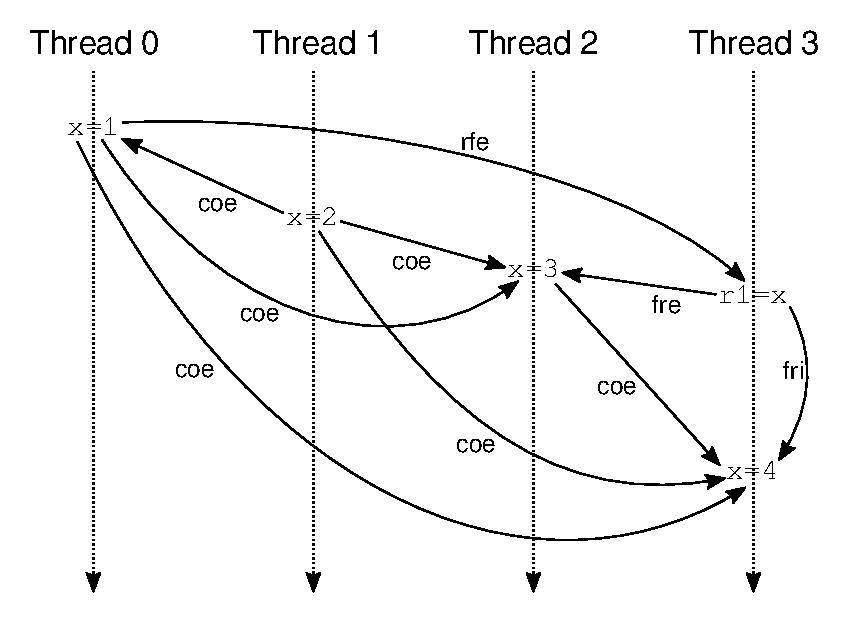
\includegraphics{ipc}}
\caption{IPC Diagram for coe, fre, and rfe}
\label{fig:IPC Diagram for coe, fre, and rfe}
\end{center}
\end{figure}

Thirdly, Figure~\ref{fig:IPC Diagram for coe, fre, and rfe} illustrates
the coe, fre, fri, and rfe links for four threads with time advancing
from the top to the bottom of the figure.  Starting with coe, even though
Thread~1's store was later in global time than that of Thread~0, that of
Thread~1 came first in coe order, followed by those of Threads~2 and ~3.
There is thus a coe link from Thread~1's store to every other store,
from Thread~0's store to those of Threads~2 and~3, and from Thread~2's
store to that of Thread~3.
This situation can occur due to the initial placement and subsequent
movement of cache lines.

Thread~3's load reads the value stored by Thread~0's store, so there is
an rfe link from that store to that load.  There is also an fre link from
that load to Thread~2's store and an fri link to Thread~3's later store.
Note that this fre link goes backwards in time.

Finally, there might be a desire for hard evidence that coe and fre
links really can go backwards in time.
We provide this evidence on x86 to demonstrate that these effects
are not confined to weakly ordered systems.
This system is a dual-socket system with
Intel(R) Xeon(R) Gold 6138 CPU @ 2.00GHz,
each socket with 20~cores, each having a pair of hardware
threads, for a grand total of 80 hardware threads.
The code generating this data may be found in the \path{CodeSamples/cpu}
directory of the
perfbook~\cite{McKenney2018ParallelProgramming-2018-12-08a}.\footnote{
	\co{git clone git://git.kernel.org/pub/scm/linux/kernel/git/paulmck/perfbook.git}}

\begin{figure}[tb]
\begin{center}
\resizebox{4in}{!}{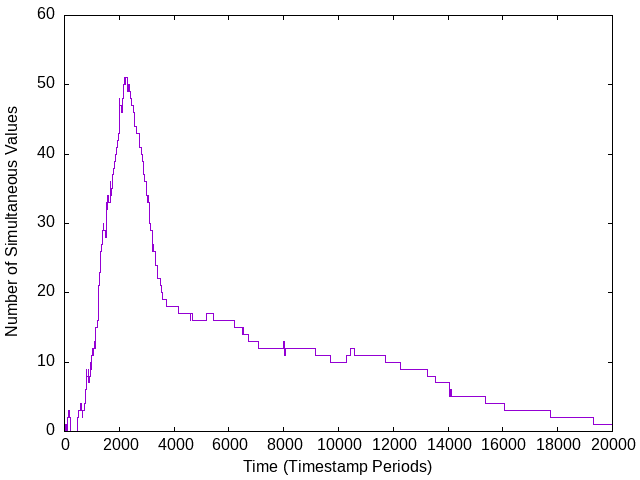
\includegraphics{coe-nvals}}
\caption{On x86, Reasonable CPUs Can Disagree}
\label{fig:On x86; Reasonable CPUs Can Disagree}
\end{center}
\end{figure}

Figure~\ref{fig:On x86; Reasonable CPUs Can Disagree}
shows the results of 79 of the systems's hardware threads simultaneously
storing their identifying integer (ranging from 0 to 78) to a shared
variable, then repeatedly doing timestamped reads from that variable.
The x-axis displays time in TSC periods, each of which is about 0.5~ns
in duration.
The y-axis shows the number of distinct opinions that the hardware
threads have as a function of time, a number that is frequently rather
larger than one.
The backwards-in-time coe link from Thread~1 to Thread~0 in
Figure~\ref{fig:IPC Diagram for coe, fre, and rfe}
is therefore entirely plausible.

\begin{figure}[tb]
\begin{center}
\resizebox{4in}{!}{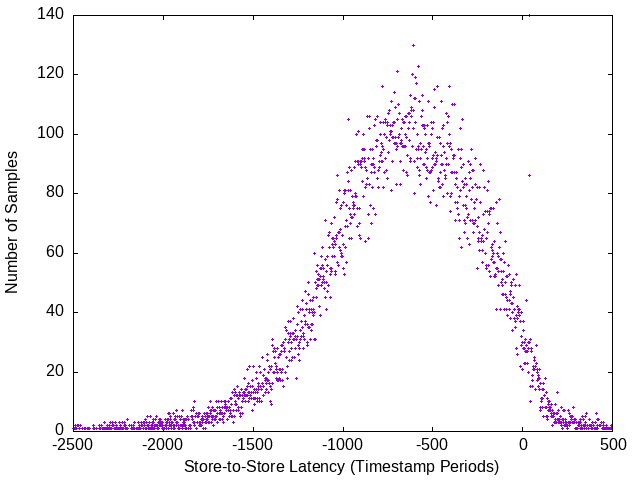
\includegraphics{coe-sh-out}}
\caption{On x86, coe Links Are Atemporal}
\label{fig:On x86; coe Links Are Atemporal}
\end{center}
\end{figure}

Not only is this plausible, but as you can see in
Figure~\ref{fig:On x86; coe Links Are Atemporal},
it actually happens, and frequently.
The store-to-store latency is measured from the end of the ``winning''
store to the beginning of the non-winning store that started latest.
Every data point on the negative x-axis represents a group of runs
in which the winning store was not the last store.
Thus, the winning store not being the last store is quite common, even
on x86.

\begin{figure}[tb]
\begin{center}
\resizebox{5in}{!}{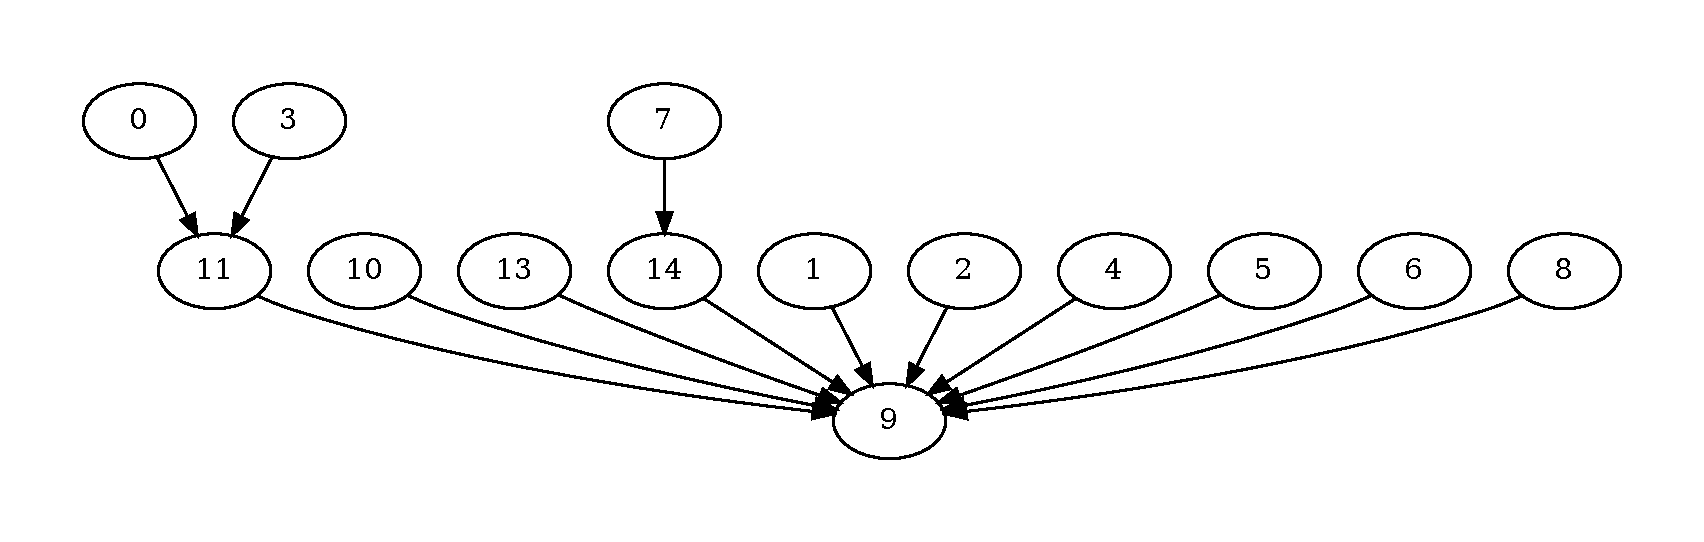
\includegraphics{coe-out-1}}
\caption{On x86, coe Links Are Partially Ordered}
\label{fig:On x86, coe Links Are Partially Ordered}
\end{center}
\end{figure}

\begin{figure}[tb]
\begin{center}
\resizebox{3in}{!}{\rotatebox{90}{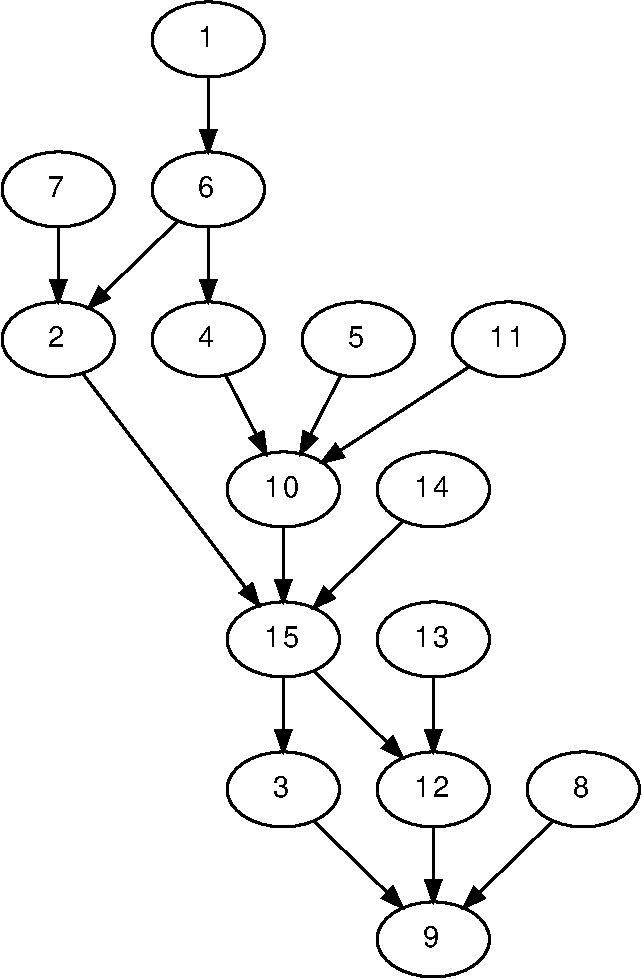
\includegraphics{store15tred}}}
\caption{On Power5, coe Links Are Also Partially Ordered}
\label{fig:On Power5, coe Links Are Also Partially Ordered}
\end{center}
\end{figure}

However, Figure~\ref{fig:On x86, coe Links Are Partially Ordered}
shows that the order of reads of each value at each thread are
consistent with a number of global orders, as required.\footnote{
	Taken on a 16-CPU x86 laptop to avoid an unreadable
	diagram containing 79 bubbles.}
Figure~\ref{fig:On Power5, coe Links Are Also Partially Ordered}
shows a rather more elaborate partial order from a Power5
system~\cite{McKenney2018ParallelProgramming-2018-12-08a}.

\begin{figure}[tb]
\begin{center}
\resizebox{3in}{!}{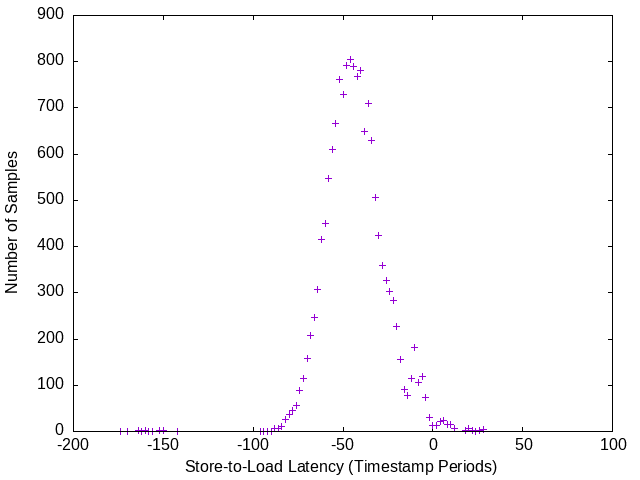
\includegraphics{fre-sh-out}}
\caption{On x86, fre Links Are Atemporal}
\label{fig:On x86, fre Links Are Atemporal}
\end{center}
\end{figure}

Figure~\ref{fig:On x86, fre Links Are Atemporal}
plots a histogram of the elapsed time from the beginning of load to
return the old value to the end of the store that provided the new value.
Note well that most of the data falls into negative time, that is to
say, in the most commonly occurring case, the last load of the old value
executes about 60 timestamp periods (about 30~nanoseconds) \emph{after}
the store that overwrote that same old value.
That is, fre links can and do go backwards in time.
This corresponds to the fre link between Thread~3 and Thread~2 depicted in
Figure~\ref{fig:IPC Diagram for coe, fre, and rfe}.

\begin{figure}[tb]
\begin{center}
\resizebox{3in}{!}{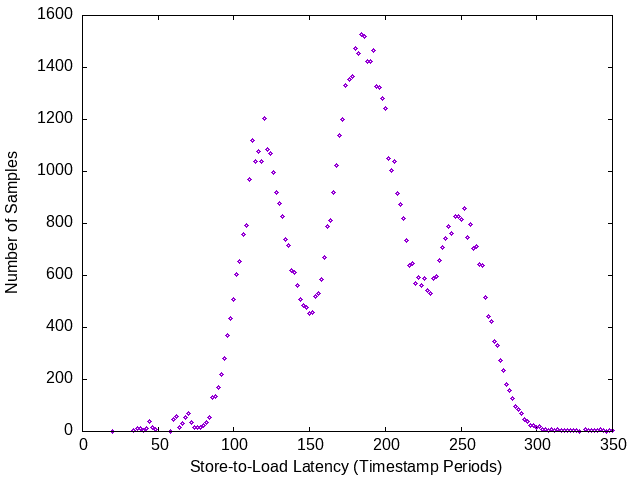
\includegraphics{rfe-sh-out}}
\caption{On x86, rfe Links Are Temporal}
\label{fig:On x86, rfe Links Are Temporal}
\end{center}
\end{figure}

Figure~\ref{fig:On x86, rfe Links Are Temporal}
plots a histogram of the elapsed time from a store of a new value
to the first load of that new value.
Note well that all of the data falls into positive time, indicating
that rfe links always go forward in time, as those familiar with
computer hardware and the laws of physics would expect.

\begin{figure}[tb]
\begin{center}
\resizebox{4in}{!}{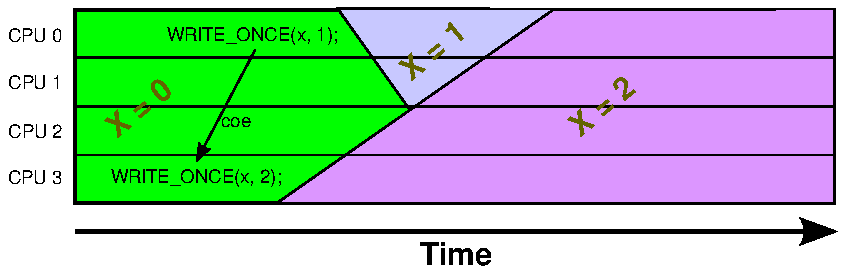
\includegraphics{coe}}
\resizebox{4in}{!}{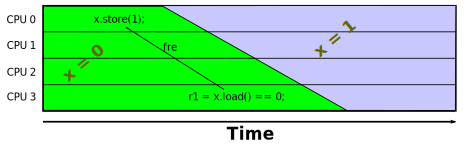
\includegraphics{fre}}
\resizebox{4in}{!}{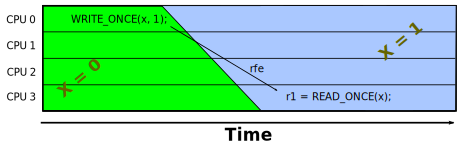
\includegraphics{rfe}}
\caption{Propagation Delay and Temporal Properties of coe, fre, and rfe}
\label{fig:Propagation Delay and Temporal Properties of coe, fre, and rfe}
\end{center}
\end{figure}

Figure~\ref{fig:Propagation Delay and Temporal Properties of coe, fre, and rfe}
shows how the temporal properties of coe, fre, and rfe are explained
by propagation delay.
In the case of coe, the two stores take time to propagate across the
system, and their ordering can be and often is decided after the fact.
In the case of fre, the store again takes time to propagate across
the system, and so a load might execute later in global time than
did the store, but not late enough to return that store's value.
In the case of rfe, the load cannot return a given store's value until
the value has propagated to that part of the system executing that load.

And this is exactly why the C++ memory model guarantees ordering from
rfe links but not the coe and fre links for relaxed accesses in the
absence of other ordering from stronger atomic memory accesses or
\co{atomic_thread_fence(memory_order_seq_cst}.

\clearpage

\section{User Influence Over Language Semantics}
\label{app:User Influence Over Language Semantics}

As noted earlier, the exact definition of a computer language is subject
to some debate, with standards, implementations, and users all having
some degree of
influence~\cite{KayvanMemarian2016DepthOfC-1,KayvanMemarian2016DepthOfC-2},
and each of which is subject to change over time.
It is natural to dismiss user influence when compared to the text of
standards or the code in implementations, but both are subject to
change and do change over time.
The implementation is especially subject to change, for example,
consider the following command line used to build the Linux kernel's
\co{kernel/rcu/tree.c} C-language source file:

~\\
{
	\scriptsize
	\texttt{
	gcc -Wp,-MMD,kernel/rcu/.tree.o.d -nostdinc
	-I./arch/x86/include \\
	-I./arch/x86/include/generated  -I./include
	-I./arch/x86/include/uapi \\
	-I./arch/x86/include/generated/uapi
	-I./include/uapi -I./include/generated/uapi \\
	-include ./include/linux/compiler-version.h
	-include ./include/linux/kconfig.h \\
	-include ./include/linux/compiler\_types.h -D\_\_KERNEL\_\_
	-fmacro-prefix-map=./= \\
	-Werror -std=gnu11 -fshort-wchar
	-funsigned-char -fno-common -fno-PIE \\
	-fno-strict-aliasing -mno-sse
	-mno-mmx -mno-sse2 -mno-3dnow -mno-avx \\
	-fcf-protection=branch
	-fno-jump-tables -m64 -falign-jumps=1 -falign-loops=1 \\
	-mno-80387 -mno-fp-ret-in-387 -mpreferred-stack-boundary=3
	-mskip-rax-setup \\
	-mtune=generic -mno-red-zone -mcmodel=kernel
	-Wno-sign-compare \\
	-fno-asynchronous-unwind-tables
	-mindirect-branch=thunk-extern \\
	-mindirect-branch-register
	-mindirect-branch-cs-prefix -mfunction-return=thunk-extern
	-fno-jump-tables -fpatchable-function-entry=16,16
	-fno-delete-null-pointer-checks -O2 \\
	-fno-allow-store-data-races
	-fstack-protector-strong -fomit-frame-pointer \\
	-fno-stack-clash-protection -falign-functions=16
	-fno-strict-overflow -fno-stack-check \\
	-fconserve-stack
	-Wall -Wundef -Werror=implicit-function-declaration \\
	-Werror=implicit-int -Werror=return-type -Werror=strict-prototypes \\
	-Wno-format-security -Wno-trigraphs -Wno-frame-address
	-Wno-address-of-packed-member \\
	-Wframe-larger-than=2048 -Wno-main
	-Wno-unused-but-set-variable \\
	-Wno-unused-const-variable -Wvla
	-Wno-pointer-sign -Wcast-function-type \\
	-Wno-array-bounds
	-Wno-alloc-size-larger-than -Wimplicit-fallthrough=5 \\
	-Werror=date-time -Werror=incompatible-pointer-types
	-Werror=designated-init \\
	-Wenum-conversion
	-Wno-unused-but-set-variable -Wno-unused-const-variable \\
	-Wno-restrict -Wno-packed-not-aligned -Wno-format-overflow
	-Wno-format-truncation \\
	-Wno-stringop-overflow
	-Wno-stringop-truncation -Wno-missing-field-initializers \\
	-Wno-type-limits -Wno-shift-negative-value
	-Wno-maybe-uninitialized \\
	-Wno-sign-compare
	-DKBUILD\_MODFILE='"kernel/rcu/tree"'
	-DKBUILD\_BASENAME='"tree"' \\
	-DKBUILD\_MODNAME='"tree"' -D\_\_KBUILD\_MODNAME=kmod\_tree \\
	-c -o kernel/rcu/tree.o kernel/rcu/tree.c
	}
}

We do not propose to explain all of these, and sufficiently motivated
readers can avail themselves of the GCC documentation.
We instead look at representative members of several categories.

The \co{-funsigned-char} causes type \co{char} to be unsigned, which
overrides per-architecture defaults, some of which treat \co{char}
as signed and others as \co{unsigned}.
This choice prevents a class of bugs, and also allows the kernel to make
reliable use of the uppermost bit of variables of type \co{char}.
It also affects the definition of ``semantic dependency'' by changing
the arithmetic proporties of this type.
In theory, the standard could specify the signedness of \co{char}, but the
variety of existing practice in the 1980s prevented this.
Plus machine instructions were much more expensive back then, so the
signedness of \co{char} was much more of a performance concern than
it is toda than
it is todayy.

The \co{-mno-sse} prevents GCC from making use of the SSE hardware.
This is done for performance reasons, as it avoids the overhead of
saving and restoring the state of this hardware when switching between
user and kernel contexts.
Similarly, the \co{-mcmodel=kernel} causes the kernel binary to be
placed in the uppermost 2GB of the address space, again reducing
the overhead of switching between user and kernel contexts.
These are cases where the standard does not specify anything, nor
should it.

The \co{-fpatchable-function-entry=16,16} causes GCC to emit 16
\co{nop} instructions at the beginning of each function, with
the function's entry point being just after this string of \co{nop}
instructions.
The resulting buffers are used by the Linux-kernel tracing infrastructure
which is in turn used for debugging, performance measurement, and
monitoring.
This is again clearly outside of the scope of the standard.

The \co{-fstack-protector-strong} causes GCC to emit code that provides
some protection against some clases of attacks based on buffer overflows.
One could rightly argue code should simply avoid ever overflowing buffers,
but things like memory allocators and userspace memory accesses must
use code that can be difficult to distinguish from buffer overflows.
It is not clear that the ever-increasing variety of attacks should
affect the standard.

The \co{-fno-strict-overflow} causes GCC to act as if signed integer
overflow is defined behavior.
Note well that this command-line option also affects the definition of
``semantic dependency''.
This might be a controversial choice, and another option would be to add
a new set of signed integer types to the standard for which overflow is
defined as wrapping, similar to the situation with unsigned integers.

The \co{-Werror=strict-prototypes} causes GCC to warn if old-style
non-ANSI function prototypes are used.
This helps avoid certain classes of bugs.
Warnings are by design outside of the scope of the standard.

In other words, user preference can exert a non-trivial influence over
language semantics, and in particular can affect some aspects of the
definition of ``semantic dependency''.

\clearpage

\section{But What About Tooling?}
\label{sec:But What About Tooling?}

This paper focuses primarily on showing that, under commonly occurring
constraints, OOTA cycles cannot form in real-world C++ implementations.

But what about tooling?

One entirely reasonable reaction is that, given the issues raised in
Sections~\ref{sec:Properties of Semantic Dependencies}
and~\ref{sec:The Fundamental Property of Semantic Dependencies},
load/store reordering is the least of the problems faced by tooling.
Nevertheless, this appendix expands on
Section~\ref{sec:Semantic Dependencies and Tooling}
by looking into the possibility of:

\begin{enumerate}
\item	Tooling focusing on only part of the language,
\item	Changing the language to eliminate some aspects that are
	troublesome for tooling (and potentially accepting performance
	and energy-efficiency shortfalls), and
\item	Changing the language to better delineate those portions that
	tooling can easily accommodate.
\end{enumerate}

But first, the next section looks at why some weakly ordered
implementations appear to forbid reordering of prior relaxed loads with
later relaxed stores,\footnote{
	Or, in memory-order-speak, forbid all load-buffering litmus tests.}
despite the architecture permitting such reordering.

\subsection{Load/Store Ordering: Hardware View for Software Hackers}
\label{sec:Load/Store Ordering: Hardware View for Software Hackers}

% @@@ Get citations

Both the ARM and PowerPC memory models permit reordering prior loads
against subsequent stores, but actual tests on recent hardware fail to
produce any evidence of any such reordering.
Nevertheless, thus far neither ARM nor PowerPC hardware architects
have been willing to strengthen their memory models so as to forbid
such reordering.
% @@@ Cite Grisenthwaite

This appendix offers some possible reasons for this odd juxtaposition
of negative test results and flat refusal.

One key point is that some hardware (including ARM and PowerPC) provides
precise exceptions.
For example, if a given load results in a segmentation violation
exception, that exception will occur before any instructions following
that load have committed.
This means that a given load instruction's execution must have proceeded
beyond the point where an exception might occur before any subsequent
store can be permitted to commit, even if that store is completely
unrelated to that load.
For example, the later store cannot commit until all prior loads' address
translations have completed successfully.

However, if that load suffers a cache miss, address translation will have
completed long before the load returns its value, meaning that a later
store might well commit before the load completes.
In fact, that later store might commit before the store that supplies the
value returned by that load!
Which explains why some hardware systems really do reorder prior loads
and later stores.

The question then becomes ``Why would weakly ordered systems fail to
reorder prior loads with later stores?''

One explanation is ECC errors.

If correctable ECC errors were fixed up in hardware, then only uncorrectable
ECC errors would be directly visible to software.
If the only possible reaction to an uncorrectable ECC error was to
terminate the program suffering that ECC error, it would be safe to
allow subsequent stores to commit as soon as all prior loads' address
translations had completed successfully.

However, some kernels and applications have ways of handling even
uncorrectable errors.
Operating-system kernels encountering an ECC error might note that the
affected data was being used by only one user process, and might react by
killing that user process, taking care to account for memory shared with
other processes.
Some user applications might be note that the affected data affected only
a particular computation, and might react by restarting that computation.
In both cases, it is only reasonable to react to an uncorrectable ECC
error in a load from a read-only mapped file by re-reading that data
from that file, then restarting that load instruction.
In all cases, the kernel and the user application would need to continue
execution, and would thus require an exact exception.

Systems that offload processing of correctable ECC errors to software
also require exact exceptions.
After all, the software is going to need to be able to correct the error
and then fix up the state to make it appear that the load had returned
the fixed-up value.

ECC errors are detected near the end of their corresponding load
instructions' execution, so that any need for exact exceptions rules out
the commiting of any subsequent stores until after the load has fetched
(and possibly corrected) its value.

So why are hardware architects reluctant to tighten their memory models
to forbid reordering of earlier loads and later stores?

If you would like an authoratative answer to this question, you should of
course ask your friendly local hardware architect.
In the meantime, here is some semi-informed speculation on this topic:

\begin{enumerate}
\item	Some hardware might choose to forego ECC, for example, in order to
	reduce cost for low-end systems or to improve energy efficiency
	for battery-powered systems.
\item	ECC error correction might still be done in hardware, avoiding
	the need for precise software-visible exceptions.
\item	Some systems might prefer to immediately shut down in response to
	an uncorrectable ECC error, perhaps due to safety considerations.
	This would entirely avoid the need for software-visible
	ECC-related exceptions.\footnote{
		One motivation for immediate shutdown is that if there
		are uncorrectable errors, there might soon be errors
		that translate one valid bit pattern to another valid
		bit pattern, which could result in a lack of safety.}
\item	Someone might come up with a clever way of correcting ECC errors
	in firmware, avoiding the need for precise software-visible
	exceptions.
\item	As late as early 2024, some GPGPUs have been observed reordering
	earlier loads against later stores.
	Other hardware architects might therefore feel the need to keep
	this option open for their own systems.
\end{enumerate}

So although it is not unreasonable to continue asking hardware vendors
to tighten their memory models so as to prohibit reordering of earlier
loads and later stores, it also would not be too surprising for them to
continue to refuse.

\subsection{Status Quo and Focused Tooling}
\label{sec:Status Quo and Focused Tooling}

The theoretical possibility of OOTA cycles causes some tools to have
difficulty identifying precisely which outcomes are impossible on
real-world C++ implementations.
One approach is for tooling to reject programs containing instances
of \co{memory_order_relaxed} and \co{memory_order_consume}, so that
developers desiring their code to be analyzed by such tools would
avoid using these \co{memory_order} values.
The is strong precedent for this strategy, with the common prohibition
against side effects in function arguments being but one example.

However, there is a large body of existing code that uses
\co{memory_order_relaxed}, and it would be unfortunate if such tools
could not be applied to this code.

Another approach would be to add flags to C++ implementations
to cause \co{memory_order_relaxed} to be interpreted as either
\co{memory_order_acquire} (for loads), \co{memory_order_release} (for
stores), or \co{memory_order_acq_rel} (for read-modify-write operations).
On TSO systems and on systems featuring exact ECC exceptions, this
would allow tooling to be brought to bear without performance or
energy-efficiency consequences beyond forgone optimizations involving
memory reference reordering.

However, this would mean that programs compiled in this way would not
be guaranteed to run correctly on weakly ordered systems that lack
ECC (or that lack precise exceptions).
In addition, this change is more strict than necessary, forbidding
optimizations that tooling could in fact analyze.
Therefore, the next section looks at standardizaing a less severe
restriction.

\subsection{Change Relaxed to Forbid Load Buffering}
\label{sec:Change Relaxed to Forbid Load Buffering}

Tooling does not require relaxed accesses become fully acquire and/or
release, but rather only that implemetnations be forbidden from reordering
prior relaxed loads with subsequent relaxed stores, as has been suggested
many times over the
years~\cite{Boehm:2014:OGA:2618128.2618134,HansBoehm2019OOTArevisitedAgain,Lahav:2017:RSC:3062341.3062352}.

This preserves portability while enabling tooling to handle all members
of the \co{memory_order} enumeration, but inflicts some performance and
energy-efficiency penalties~\cite{LukeGeeson2023TightenRelaxed} in
code not requiring these ordering
restrictions~\cite{PaulEMcKenney2020RelaxedGuideRelaxed}.

This suggests the addition of a \co{memory_order_load_store} member to
the \co{memory_order} enumeration, a topic taken up by the next section.

\subsection{Add Load-Store Memory Order that Forbids Load Buffering}
\label{sec:Add Load-Store Memory Order that Forbids Load Buffering}

The addition of a \co{memory_order_load_store} member to the
\co{memory_order} enumeration has been suggested starting many years
ago~\cite{HansBoehm2019OOTArevisitedAgain,DanielLustig2018PlacedBefore}.
This does not resolve all shortcomings in the C++ memory
model~\cite{PaulEMcKenney2023P0124R8-LKMM,DanielLustig2018PlacedBefore},
but it would provide a portable \co{memory_order} that minimally
restricted compiler and hardware optimizations while still permitting
full analyzability by current software tools.

This change would also leave \co{memory_order_relaxed} in place,
allowing minimal-overhead accesses in fastpaths.
These fastpaths would not be analyzable by generic tools, but could
be handled by special-case tools that analyze the binaries to verify
that required orderings are enforced by machine-language properties
such as dependencies.
And a tool that checks control dependencies has in fact been
prototyped~\cite{PaulHeidekrueger2022N4910}.

This suggests a combined strategy of adding \co{memory_order} members
as needed to extend the reach of general-purpose tooling, while also
identifying \co{memory_order_relaxed} idioms that are checked at the
machine level using special-purpose tooling.\footnote{
	Kudos to Peter Sewell for clearly articulating this possibility
	as part of an overall strategy.}

% \section{History}
% \label{sec:History}

\clearpage

\section{Acknowledgments}
\label{sec:Acknowledgments}

We are grateful to David Goldblatt, Jade Alglave, and Peter
Sewell for their careful review of an early draft of this paper and
to John Wickerson for asking Paul for a rant and taking the proffered
rant seriously.
We also owe David Goldblatt a debt of gratitude for his having asked an
insightful question at the right time, his insights on combinations of
OOTA and UB, and for his ``Deathstation 9000'' demonic CPU.
% Alan Stern located many unclear statements and gaps in reasoning.
Martin Uecker contributed valuable insights on backwards-propagating UB.
Gonzalo Brito Gadeschi shared an alternative way of handling non-volatile
atomic operations.
Richard Grisenthwaite patiently explained the architectural constraints
that prevent hardware OOTA.

Nonetheless, all errors and omissions in this paper are the sole property
of the authors, and the appearance of a name in this appendix does
not in any way constitute agreement with anything in this paper.

% @@@ reviewer to do.
% Luc Maranget: Memory models.
% Greg Kroah-Hartman and Linus Torvalds: FYI, trouble being caused.
% Christoph Hellwig: Why slow on BPF memory model.
% Miguel Ojeda: LKMM and Rust.
% Alice Ryhl: LKMM and Rust.
% Ralf Jung: Rust.
% Catalin Marinas: ARM and formal methods (qspinlock).
% Segher Boessenkool:  GCC.
% Dan Lustig: NVIDIA memory ordering.
% Andrea Parri: Memory models, RISC-V hardware.
% Jonas Oberhauser: Memory models.
% Hernan Ponce de Leon: Memory models.
% Palmer Dabbelt: RISC-V hardware.
% Ali Sezgin: P0422R0.
% Tony Tye: P0422R0.
% Other memory-model maintainers.
% Derek Williams: PowerPC hardware.
% Hans Boehm: Skeptic, memory models, OOTA.  Suggestions for others?
% Olivier Giroux: Skeptic, memory models, NVIDIA.
% Luke Geeson: Whatever...  Review.
% Ori Lahav: Prior OOTA.
% Viktor Vafeiadis:  Prior OOTA.
% Derek Dreyer: Prior OOTA.
% Brian Demsky: Prior OOTA.

% Done as of December 18, 2023:
% David Goldblatt
% Boqun Feng, Uladzislau Rezki, Neeraj Upadhyay, Joel Fernandes, and
%	Frederic Weisbecker (RCU proteges)
% Michael Wong
% Maged Michael
% John Wickerson: Thank you.  OK for Peter Sewell, Mark Batty, etc.
% Akira Yokosawa: Professional courtesy, perfbook memory models.
% Dan Kelley, Alexei Starovoitov, Mykola Lysenko: FYI.  OOTA dropped
% Alan Jeffrey: Fixed-point insight P0422R0.  Reached out via LinkedIn.
% Jade Alglave: C++ herd model?  Memory models and variety of hardware.
% Alan Stern: Memory models, mathematical logic, and variety of hardware.
% Martin Uecker (offered)
% Peter Sewell
% Mark Batty
% Richard Gristenthwaite: ARM hardware.  Posed HW speculation question.
% Peter Zijlstra.
% Mark Rutland: ARM memory ordering.
% Will Deacon: ARM hardware, C++, and OOTA.

% @@@ TODO:
% Construct interleaved OOTA examples (see sheets of paper).
% Use LKMM as check for dependencies?

% Objections:
% "Atomic operations are not observable behavior."
%	They are for volatile atomic objects.  Plus an implementation
%	whose analysis is confined to a thread would need to assume
%	that any atomic store might lead to observable behavior in some
%	other thread.  An implementation with a global view must preserve
%	observable behavior regardless of OOTA cycles.	Plus if an OOTA
%	cycle does not affect observable behavior, who cares?
% "The C++ abstract machine is independent of the laws of physics."
%	That might be, but any real implementation of that abstract
%	machine will be governed by those laws.
% "Real hardware can exhibit OOTA, as exemplified by audio feedback."
%	Such hardware does not run C++.  Also, audio feedback is more
%	closely approximated by a loop calculating sound intensity than
%	by OOTA, especially given that you must include the audio
%	properties of the enclosing space in analyzing the feedback loop.

% Additional snark:
% "This work reduces the problem of OOTA analysis to that of sequential
%	program analysis.  If you expect better verification of concurrent
%	code than of sequential code, you are in an intellectual state
%	of sin."
% "Forcing relaxed loads to be ordered before subsequent relaxed stores
%	is an expensive no-op."
% "So you don't want to learn concurrency?  Then I can only suggest
%	that you either move further up the stack or take early
%	retirement."  Note that that C++ committee's concurrency
%	expertise has grown beyond recognition over the past 15 years.

% One-pager:
% Threats to validity:
% Speed of light might not always be finite.
% Zero-sized atoms might be discovered.
% It might be possible to propagate information at infinite velocity
%	despite the finite speed of light.
% It might be possible to violate causality.
% Hardware and compiler bugs might result in OOTA.
% ML hallucination might convince people that OOTA is OK.

\bibliographystyle{plain}
\bibliography{bib/RCU,bib/WFS,bib/hw,bib/os,bib/parallelsys,bib/patterns,bib/perfmeas,bib/refs,bib/syncrefs,bib/search,bib/swtools,bib/realtime,bib/TM,bib/standards,bib/memorymodel.bib}

\end{document}
